% Welcome! This is the unofficial University of Udine beamer template.

% See README.md for more informations about this template.

% This style has been developed following the "Manuale di Stile"
% (Style Manual) of the University of Udine. You can find the
% manual here: https://www.uniud.it/it/ateneo-uniud/ateneo-uniud/identita-visiva/manuali-immagine-stile/manuale-stile

% Note: for some reason, the RGB values specified in the manual
% do NOT render correctly in Beamer, so they have been redefined
% for this document using the high level chromo-optic deep neural 
% quantistic technology offered by Microsoft Paint's color picker.

% We defined four theme colors: UniBrown, UniBlue, UniGold
% and UniOrange. For example, to write some uniud-brownish
% text, just use: \textcolor{UniBrown}{Hello!}

% Note that [usenames,dvipsnames] is MANDATORY due to compatibility
% issues between Madrtikz and xcolor packages.

\documentclass[usenames,dvipsnames]{beamer}
\usepackage[utf8]{inputenc}
\usepackage{verbatim}
%\usetheme{uniud}
\usetheme[progressbar=frametitle]{Boadilla}
\usecolortheme{dove}
\addtobeamertemplate{footnote}{\vspace{-6pt}\advance\hsize-0.5cm}{\vspace{6pt}}
\usepackage{amsmath,amssymb}
\usepackage{graphicx}
\usepackage{color}
\usepackage{setspace}
\usepackage[english]{babel}
\usepackage[utf8]{inputenc}
\usepackage{times}
\usepackage{tikz}
\usepackage{lipsum}%
\usepackage{amsmath}
\usepackage{lastpage}
\usepackage{verbatim}
\usetikzlibrary{calc,arrows,shapes,positioning}
\usepackage{color,soul}
\usepackage{booktabs }
\usepackage{algorithm,algorithmic}
\usepackage{tikz,pgfplots}
\usepackage{mathptmx}
\usepackage[scaled=.90]{helvet}
\usepackage{courier}
\usepackage[absolute,overlay]{textpos}
\usepackage{graphicx}
\usepackage{booktabs}
\usepackage{units}
\usepackage{subfigure}
\usepackage{float}
\usepackage{array}
\usepackage{environ}
\usepackage{esint}
\usepackage{hyperref}
\usepackage{ragged2e}
\usepackage[autoplay,autoresume]{animate}
\usepackage[font={small,it}]{caption}
 \usepackage{subfigure} % subfiguras
\usepackage{lipsum}% http://ctan.org/pkg/lipsum
\usepackage{hanging}% http://ctan.org/pkg/hanging
\usepackage[style=authoryear,backend=biber]{biblatex}
\usepackage{pgfplots}
\usepackage{footmisc}
\usepackage{etoolbox}

\addbibresource{bibliography.bib}

\BeforeBeginEnvironment{theorem}{
    \setbeamercolor{block title}{fg=black,bg=orange!50!white}
    \setbeamercolor{block body}{fg=orange, bg=orange!30!white}
}
\AfterEndEnvironment{theorem}{
 \setbeamercolor{block title}{use=structure,fg=structure.fg,bg=structure.fg!20!bg}
 \setbeamercolor{block body}{parent=normal text,use=block title,bg=block title.bg!50!bg, fg=black}
}
%%% Suppress biblatex annoying warning
\usepackage{silence}
\WarningFilter{biblatex}{Patching footnotes failed}

%%% Some useful commands
% pdf-friendly newline in links
\newcommand{\pdfnewline}{\texorpdfstring{\newline}{ }} 
% Fill the vertical space in a slide (to put text at the bottom)
%\newcommand{\framefill}{\vskip0pt plus 1filll}

\usepackage{lipsum}% http://ctan.org/pkg/lipsum
\usepackage{hanging}% http://ctan.org/pkg/hanging

\let\oldfootnote\footnote
\renewcommand\footnote[1][]{\footnotesize\oldfootnote[frame,#1]}
\renewcommand{\footnotesize}{\tiny}
\renewcommand{\footnoterule}{%
\kern 2pt
}

\definecolor{UniRed}{RGB}{166,28,49}

\setbeamertemplate{section page}
{
    \begingroup
    \begin{beamercolorbox}[sep=18pt,center]{section title}
        \usebeamerfont{section title}\insertsection\par
    \end{beamercolorbox}
    \endgroup
}
% Add support for \subsubsectionpage
\def\subsubsectionname{\translate{Subsubsection}}
\def\insertsubsubsectionnumber{\arabic{subsubsection}}
\setbeamertemplate{subsubsection page}
{
%  \begin{centering}
%    {\usebeamerfont{subsubsection name}\usebeamercolor[fg]{subsubsection name}\subsubsectionname~\insertsubsubsectionnumber}
%    \vskip1em\par
%    \begin{beamercolorbox}[sep=4pt,center]{part title}
%      \usebeamerfont{subsubsection title}\insertsubsubsection\par
%    \end{beamercolorbox}
%  \end{centering}
}
\def\subsubsectionpage{\usebeamertemplate*{subsubsection page}}

\AtBeginSection{\frame{\sectionpage}}
\AtBeginSubsection{\frame{\subsectionpage}}
\AtBeginSubsubsection{\frame{\subsubsectionpage}}




\PassOptionsToPackage{demo}{graphicx}

\makeatletter
\newcommand\titlegraphicii[1]{\def\inserttitlegraphicii{#1}}
\titlegraphicii{}
\setbeamertemplate{title page}
{
  
  \begin{centering}
    \begin{beamercolorbox}[sep=8pt,center]{institute}
      \usebeamerfont{institute}\insertinstitute
    \end{beamercolorbox}
    \begin{beamercolorbox}[sep=8pt,center]{title}
      \usebeamerfont{title}\inserttitle\par%
      \ifx\insertsubtitle\@empty%
      \else%
        \vskip0.25em%
        {\usebeamerfont{subtitle}\usebeamercolor[fg]{subtitle}\insertsubtitle\par}%
      \fi%     
    \end{beamercolorbox}%
    \vskip1em\par
    \begin{beamercolorbox}[sep=8pt,center]{date}
      \usebeamerfont{date}\insertdate
    \end{beamercolorbox}%\vskip0.5em
    \begin{beamercolorbox}[sep=8pt,center]{author}
      \usebeamerfont{author}\insertauthor
    \end{beamercolorbox}
  \end{centering}
 % \vbox{}
   {\usebeamercolor[fg]{titlegraphic}\inserttitlegraphic\hfill\inserttitlegraphicii\par}
  %\vfill
}
\makeatother
\author{M.Sc. Ricardo Moncayo\\Advisor: Ph.D. Eduardo Romero}
\title{Presentation Title}
\subtitle{Presentation Subtile}
\institute{Departamento Ingeniería \\ Eléctrica}
\date{\today}
\titlegraphic{
\includegraphics[height=2.2cm,width=3.5cm]{graphics/cimalablogo.png}}
\titlegraphicii{
\includegraphics[height=2.5cm,width=2.5cm]{graphics/logo.png}}


\begin{document}

\begin{frame}[plain]
\maketitle
\small
{\centering\itshape \par}
\par\medskip

\end{frame}

%%%%%%%%%%%%%%%%%%%%%%%%%%%%%%%%%%%%%%%%%%%%%%%%%%%%%%%%%%%%%

\begin{frame}{Pathological examination issues}
	\begin{itemize}
	 \item Due to the heterogeneity between the normal tissue and the disease most of the morphological indicators of prognosis are not quantified
     \pause
	 \item Subjective observations are susceptible to inter and intra observer variations
      \textcolor{red}{Imagenes con kappa}	 
	 
	% \item As consequence the prognosis is prone to error
	 % tumor contour, lymphotic reaction in tumor, nuclear cytology, vascular invasion, tumor proliferation
	\end{itemize}
\end{frame}

\begin{frame}{The Suitability of a Quantitative Estimation in Pathology Workflow}
 \begin{itemize}
  \item Digital version of whole glass slide and image analysis are using to improve the diagnosis
  \pause

  \item The Quantification of morphological structures to determine the predisposition of a disease and to deliver healthcare\textcolor{red}{imagenes??}
  
  
  
 \end{itemize}
\end{frame}

\section{Quantification of Premalignant Lesions of the Gastric Mucosa - 1st case of Study}

\begin{frame}{Changes of the Normal Mucosa to Adenocarcinoma}
%\vspace{-0.8cm}
	%\begin{itemize}
%\only<1->{	\item Gastric cancer (GCa) is the fourth cause of death worldwide (Globocan,2012)}
		       
%\only<1->{	   \item Infection with Helicobacter Pylori bacteria (HP) has relationship with $80\%$ of GCa cases (Talley,2008)}

%\only<2->{\item Close to $60\%$ of the people has HP infection.}
%\only<3->{\item $~10\%$ of the people with helicobacter infection would get GCa in the future. (Hooi J.,2017;Pounder R.,1995)}



     
		
%	\end{itemize}
%\vspace{0.2cm}
\only<1->{\centering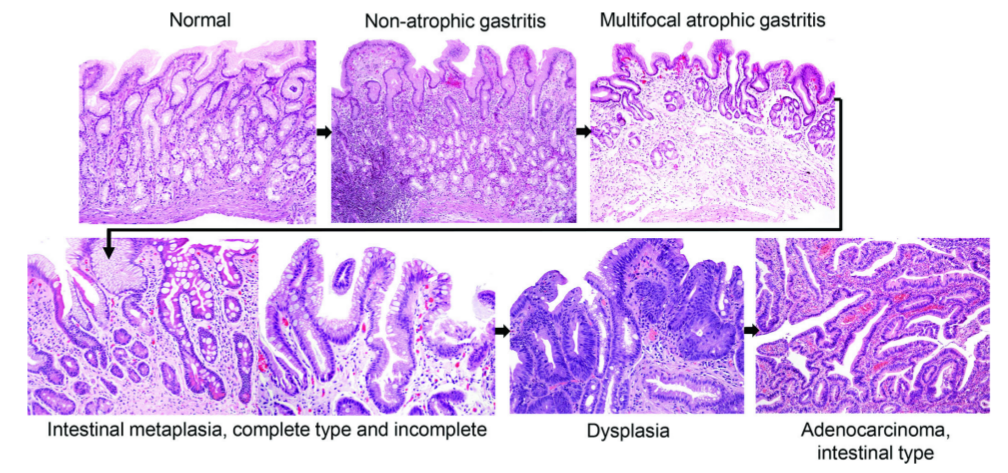
\includegraphics[width=1\textwidth]{imagenes/histopathway.png}\\
\tiny{Correa’s Cascade of Gastric Carcinogenesis;1976}}

\only<2->{\vspace{-4cm}
	\begin{alertblock}
{		\LARGE \centering Some studies suggest that the cancer progression could not follow this sequence!}
	\end{alertblock}
}
	
% \only<4>{	\begin{table}[]
% 		\centering
		
% 		\label{my-label}
% \begin{tabular}{|c|c|c|c|}
% \hline
%              $ Region \backslash n. in Thousands$                 & \textbf{Cases } & \textbf{Death} & \textbf{5-Years prevalence(survivor)} \\ \hline
% \textbf{World}                  & 952            & 723            & 1538                        \\ \hline
% \textbf{More Developed regions} & 275            & 175            & 565                         \\ \hline
% \textbf{Less Developed Regions} & 677            & 548            & 974                         \\ \hline
% \end{tabular}
% \caption{GLOBOCAN2012}
% 	\end{table}
% 		}
\footnotetext{Atrophy-metaplasia-dysplasia-carcinoma
sequence in the stomach: a reality or merely
an hypothesis?,}
\end{frame}
%  

\begin{frame}{The Carcinogenesis Cascade Main Concerns}

\begin{itemize}
 \item Diffuse type of gastric cancer are not related with atrophy or metaplasia (Lauren classification)\\
 \pause
 \item In the non-atrophic gastritis foci of intestinal metaplasia are found\footnote[1]{Stolte M, Zeitschrift f\"ur Gastroenterologie, 1992}\\

 \pause
  \item \normalsize Metaplasia grade I and II have been show no risk for cancer progression\footnote[2]{Filipe ML, International Journal of Cancer, 1994}\footnotemark[1]\\
  \pause
  \item \normalsize Dysplasia are not found in micro-early carcinomas ($Diameter < 5mm$)\footnote[3]{Hattori T.,Cancer 1986}\\
  \footnote[4]{Takizawa T, Stomach and intestine, 1998 }

  
\end{itemize}

\end{frame}
		

\begin{frame}{Inter-observer Variability}
%\subtitle{Precursor Lesions of Gastric Cancer (PGC)}
\vspace{-0.29cm}

\begin{itemize}

\only<2>{\item Kappa coefficient measure the agreement between observers, $\kappa=0$ corresponds to a bad agreement; $\kappa=1$ corresponds to a good agreement}

\only<1>{\item A highly disagreement between experts reported using kappa coeficient (Aydin,2003;Offerhaus,1999)}

\end{itemize}

\vspace{-0.24cm}
\centering
\only<1->{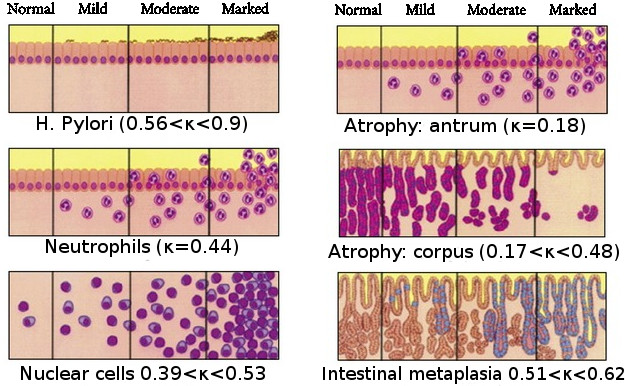
\includegraphics[width=0.56\textwidth]{imagenes/232.jpeg}
\centering \\ \vspace{-0.17cm}\tiny{Sidney analog scale}}

%}
% \begin{columns}
% \begin{column}{0.5\textwidth}
% \centering\tiny{Sidney Analog Scale}
% \includegraphics[width=1\textwidth]{imagenes/sydneyscale.jpeg}
  
% \end{column}
% \begin{column}{0.6\textwidth}  %%<--- here
%     \begin{center}
    
%      \begin{table}[]
% \centering\footnotesize
% \tiny {Agreement reports (Aydin,2003,P.2232)
% ; * (Offerhaus,1999)}
% \footnotesize
% \begin{tabular}{|c|p{1.5cm}|c|}
% \hline
% \textit{\textbf{Feature}}               & \textit{\textbf{Kappa $(\kappa)$}}                & \textit{\textbf{Interpretation}} \\ \hline
% \textit{\textbf{Atrophy in antral* }}     & 0.18                                   & poor                             \\ \hline
% \textit{\textbf{Atrophy in corpus*}}     & 0.48                                   & moderate                         \\ \hline
% \textit{\textbf{\textcolor{red}{Atrophy}}}               & 0.08-0.29, 0.17-0.57%, 0.31, 0.42, 0.51
% & poor - moderate                  \\ \hline
% \textit{\textbf{\textcolor{red}{chronic inflammation} }}  & %0.49,
% 0.39-0.53, 0.49-0.82%, 0.58%
% & poor - moderate                  \\ \hline
% \textit{\textbf{inflammatory activity}} & 0.44                                   & moderate                         \\ \hline
% \textit{\textbf{Grade of HP}}           & 0.56, %0.62, 0.74, 0.43,
% 0.9            & moderate - good                  \\ \hline
% \textit{\textbf{Intestinal metaplasia}} & 0.51-0.62, 0.54, 0.73, 0.75-0.92       & moderate - good                  \\ \hline
% \end{tabular}
% \end{table} 
%      \end{center}
% \end{column}
% \end{columns}

% Atrophy is defined as loss of
%appropriate gastric glands.
%gastric mucosal atrophy
%is considered the marker of cancer risk
%%%INFLAMATORY ACTIVITY NEUTROPHILIS
\end{frame}

\begin{frame}

\begin{alertblock}{}{
 Processes involved in gastric cancer incidence are not understood, and the current grading scales are expert dependent, A Careful and reliable measurement of histological features may prevent further malignant outcomes\footnote[5]{Tepes,2004}\footnote[6]{Sipponen P.,1994} \footnote[7]{Meining A,2001} \footnote[8]{Correa P., 1992}} 

\end{alertblock}
\end{frame}


\begin{frame}{Hypothesis}
\begin{block}{}
\centering\Large \textbf{An accurate quantification of the tissue structures will allow finding a suitable characterization of the disease}
\end{block}
\end{frame}
		
\begin{frame}{Objectives}
\textbf{General Objective:\\} 

%Formularun modelo automático para encontrar y cuantificar lesiones precursoras de malignidad en imágenes histológicas de mucosa gástrica para los diferentes grados de atrofia y metaplasia intestinal usando muestras de la población del departamento de Nariño.

 To formulate an automatic model to find and quantify patterns in gastric premalignant lesions in histological images of the gastric mucosa to the different degrees of atrophy and intestinal metaplasia\vspace{20pt}

% \textbf{Specific objetives:}

% \begin{itemize}
% \item To find structures automatically ingastric premalignant lesion in histological images such as gastric
% glands, signet ring cell, intestinal glands, fibrosis, metaplasia and dysplasia.
% \item To establish a ground truth to validate the accuracy of
% the structures finds automatically.
% \item To quantify the structures and correlate them with the
% histological concept.
% \item To validate the quantification with the diagnosis of the
% pathologist.
% \end{itemize}
\end{frame}

\begin{frame}{Contribution}
\begin{itemize}
\item The proposal consists in highlighting the importance of an exact measurement in gastric  premalignant lesions and the possibility of using this in the pathology workflow.
%\pause 
%\item To help to understand the limits between the different stages of the disease
\end{itemize} 

\end{frame}

\begin{frame}{Expected results}
\begin{itemize}
\item Different strategies to establishes the stage in PGC lesions
%\item A method to determine hidden topics in PGC
\item A computer-aided system to be applied by a pathologist in the workflow
\end{itemize}
\end{frame}

\section{Materials and Methods}
\begin{frame}{Materials}
\begin{itemize}
\item  TCGA Gastric cancer open database with 771 whole slide images and 443 of this with their histological description
\item A temporal cohort of histological images with PGC from Urkunina 5000 project
\item 30 GCa cases from Universidad Nacional de Colombia
%\item 16 GCa cases from Universidad Nacional de Colombia
%\item A server with available GPU's 
\end{itemize}

\end{frame}
%
%\begin{frame}{Methods}
%\begin{enumerate}
%\item To find and characterize normal mucosa tissue
%\end{enumerate}
%%\includegraphics[width=\textwidth,height=\textheight]{imagenes/work-in-progress.png}
%% Working on.
% \centering\includegraphics[width=0.85\textwidth]{imagenes/pipelineGC.png}
%\end{frame}
%\section{Research Group}
%


\section{Nuclear Pleomorphism (NP) in Ductal carcinoma in situ (DCIS) - 2nd case of Study}

%\section{ Nuclear Pleomorphism (NP) - The Suitability of a Quantitative Estimation}


\begin{frame}{Nuclear Pleomorphism}
\vspace{-0.5cm}
\begin{itemize}
\only<1->{\item Researching in automatic quantification strategies for nuclear pleomorphism in breast cancer(NPBca).
}
\only<2->{\item NPBca is an indicator of the aggressiveness of the disease
}
\only<3->{\item A low inter-observer agreement ($0.3<\kappa<0.5$)}
\end{itemize}

\vspace{0.3cm}
\only<1->{
\begin{columns}

\begin{column}{0.33\textwidth}
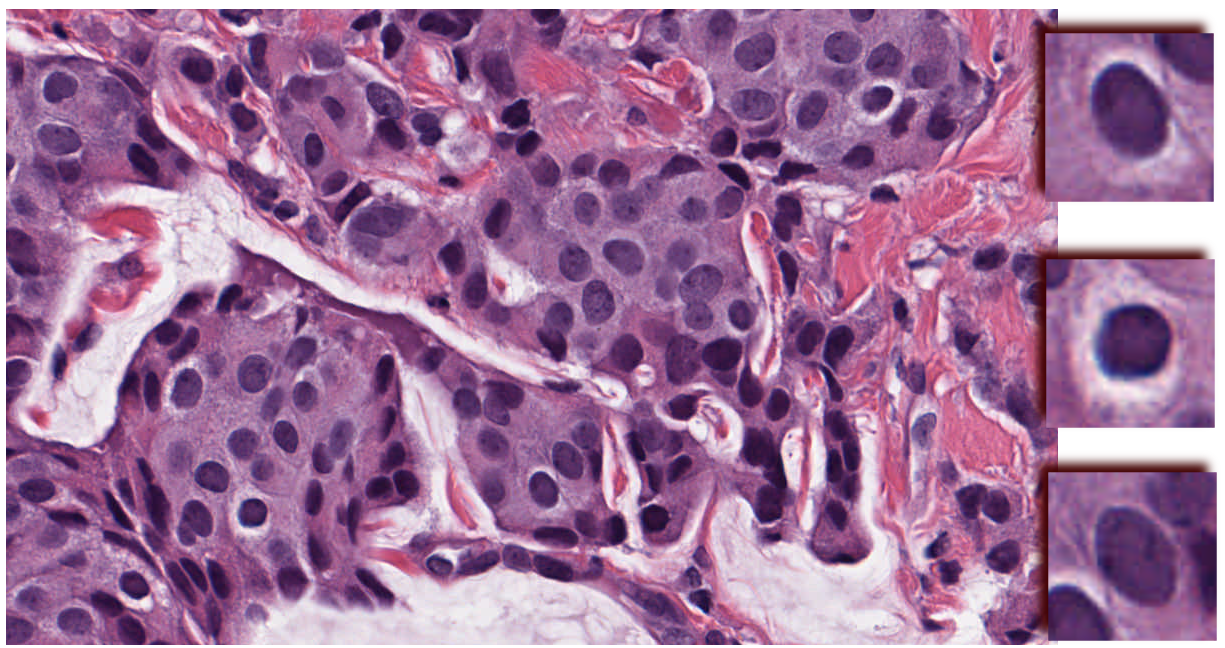
\includegraphics[width=\textwidth]{imagenes/grado1.png}
\\\centering \scriptsize grade 1

\end{column}

\begin{column}{0.33\textwidth}
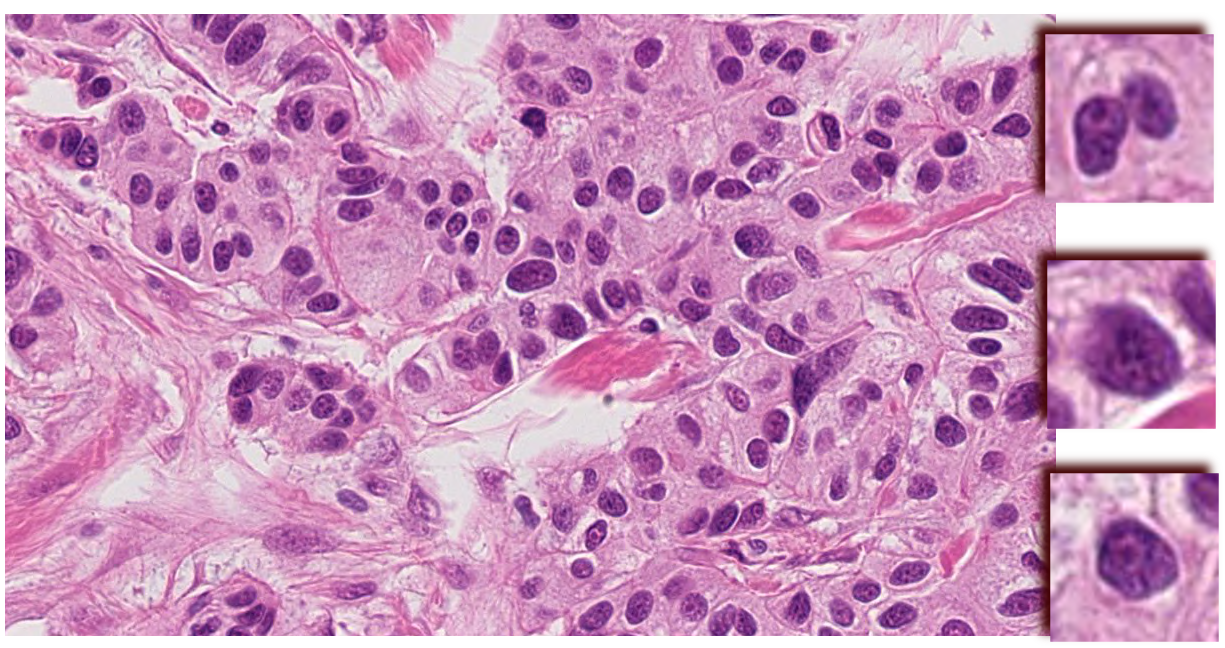
\includegraphics[width=\textwidth]{imagenes/grado2.png}
\\\centering \scriptsize grade 2

\end{column}

\begin{column}{0.33\textwidth}
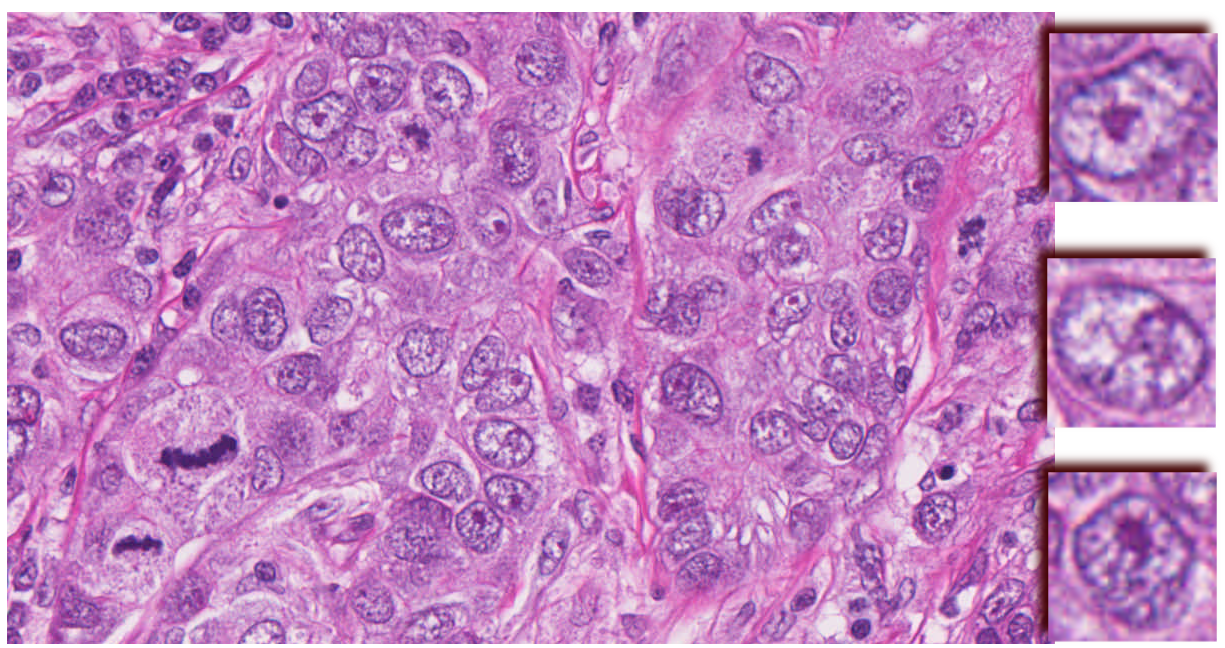
\includegraphics[width=\textwidth]{imagenes/grado3.png}
\\\centering \scriptsize grade 3

\end{column}

\end{columns}
      
  }
\end{frame}


\begin{frame}{Previous: A Bag of Features Based Strategy }
\centering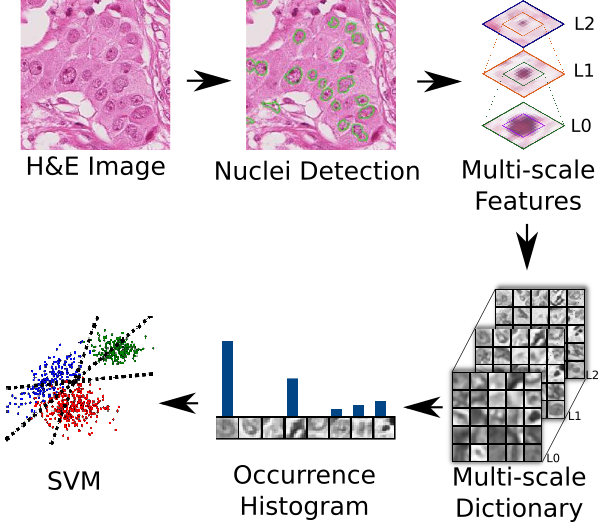
\includegraphics[width=0.57\textwidth]{imagenes/metodo_sustentacion.png}
\end{frame}
\begin{frame}{Previous: A Bag of Features onto a Graph Strategy}
%\framesubtitle{Structure Strategy}
\centering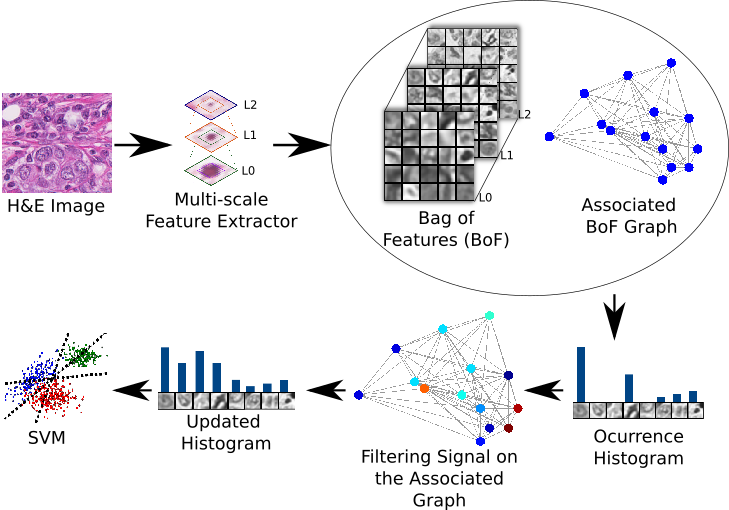
\includegraphics[width=0.68\textwidth]{imagenes/metodo_sipaim2017.png}
\end{frame}

\begin{frame}{Research Products }

\small
\begin{itemize}
\item Moncayo, R., Romo-Bucheli, D., Romero, E. \textbf{A Grading Strategy for Nuclear Pleomorphism in Histopathological Breast Cancer Images Using a Bag of Features (BOF)}. In Progress in Pattern Recognition, Image Analasys, Computer Vision and Applications, Pages 75-82, november 2015. ISBN 978-3-319-25751-8
\item Romo-Bucheli, D., Moncayo, R., Cruz, A., Romero, E., \textbf{Identifying histological concepts on basal cell carcinoma images using nuclei based sampling and multi-scale descriptors}. In 2015 IEEE 12th International Symposium on Biomedical Imaging (ISBI), April 2015, pages 1008-1011, ISSN 1945-7928
\item Moncayo, R., Romo-Bucheli, D., Arias, V., Romero, E., \textbf{Scoring Nuclear pleomorphism using a visual BoF modulated by a graph structure}, In the 13th International Symposium on Medical Information Processing and Analysis, October 2017
\end{itemize}


\end{frame}



\begin{frame}{The Next Step}
\begin{block}{}
The use of nuclear pleomorphism grade would be correlated with the patient outcome resulting in a reliable measure for the patient
\end{block}
\end{frame}

\begin{frame}{Materials}

Coming soon...

\end{frame}


\begin{frame}{Multi-scale Features}
\begin{itemize}
\item<1->\justifying Each nucleus candidate is represented by multiple scales characterized by the discrete cosine transform (DCT) using enough coefficients to reconstructing the original image
\item The coefficients from different scales are concatenated into a single feature  
\end{itemize}
\begin{figure}
\hspace{-4.5cm}\includegraphics<1->[width=7cm]{imagenes/descriptor.jpg}
\end{figure}
 \begin{textblock}{20}(9,10)
  \onslide<2->{$F(X_i)=\lbrace DCT(L0),DCT(L1),DCT(L2)\rbrace$}
 \end{textblock}
\end{frame}

\begin{frame}{Probabilistic Latent Semantic Analysis(PLSA)}
\begin{itemize}
\item Each multiscale representation is used as a \textbf{document} for build a PLSA model to find some topics
\pause
\item T-sne is used to visualize the original space and the PLSA generated
\end{itemize}
\end{frame}

\begin{frame}{Visual Results - Original Space}
\centering
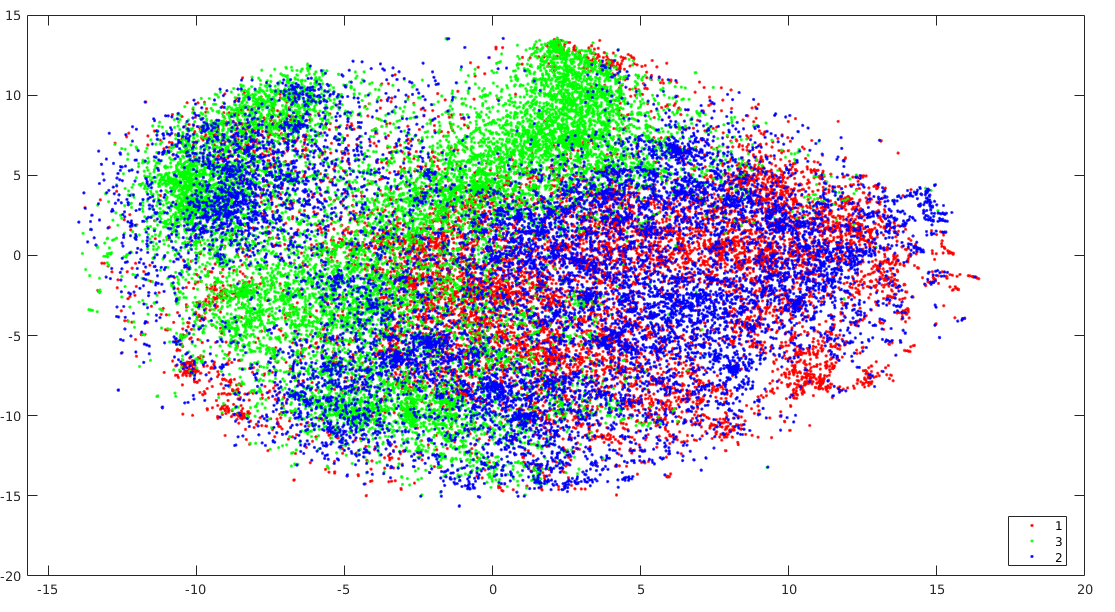
\includegraphics[width=0.85\textwidth]{imagenes/all.png}
\end{frame}

\begin{frame}{Visual Results - Space by topic}
\vspace{-0.45cm}
\begin{table}[]
\begin{tabular}{ll}
 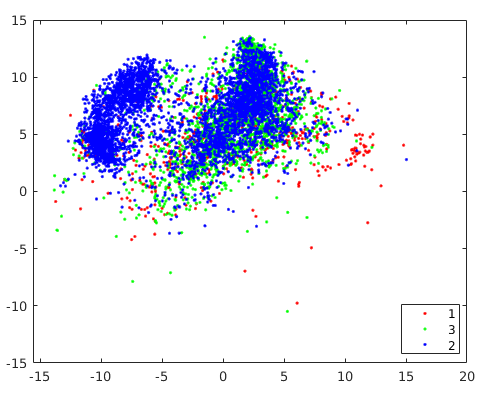
\includegraphics[width=0.31\textwidth]{imagenes/cluster3.png}& 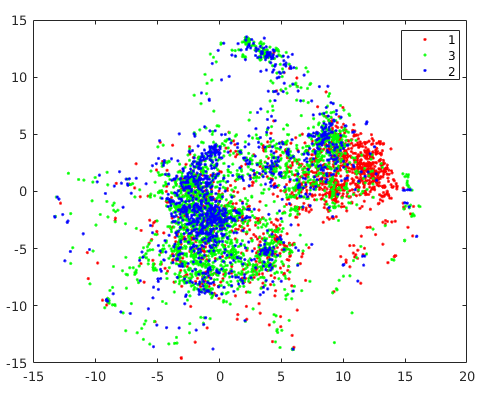
\includegraphics[width=0.31\textwidth]{imagenes/cluster4.png} \\
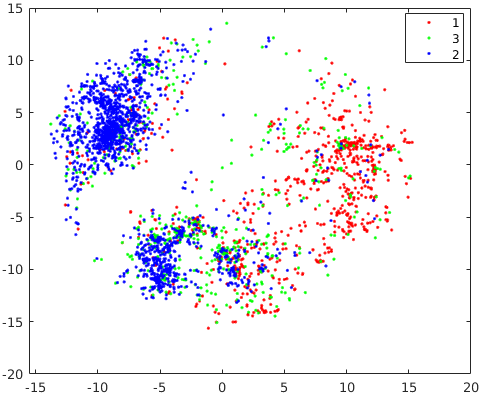
\includegraphics[width=0.31\textwidth]{imagenes/cluster8.png} & 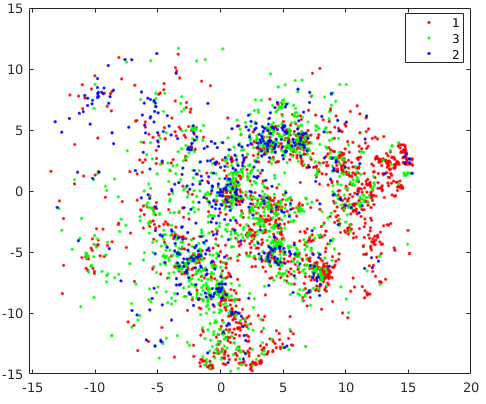
\includegraphics[width=0.31\textwidth]{imagenes/clustes7.png}
\end{tabular}
\end{table}

\end{frame}


\begin{frame}{Research Group}
\vspace{0.5cm}
\begin{columns}
\begin{column}{0.2\textwidth}

\includegraphics[width=\textwidth]{graphics/cimalablogo.png}
\end{column}
\begin{column}{0.8\textwidth}
The Computer Imaging and Medical Applications Laboratory (CIM@LAB) is a research group devoted to solve pertinent medical problems by combining artificial vision and machine learning techniques.
\end{column}
\end{columns}

\begin{columns}
\begin{column}{0.33\textwidth}
\onslide<2->{\textbf{Classification:} A1\\
\textbf{Director:} Ph.D Eduardo Romero\\
\textbf{Professors:} 2\\
\textbf{Doctoral Students:} 9\\
\textbf{Master Students:} 19\\
}
\end{column}
\begin{column}{0.33\textwidth}

\begin{itemize}
\item<3-> Digital anatomy through images
\item<4->  Digital Pathology
\item<5->  Motion and bio-signal analysis
\item<6->  Medical information systems and technology
\end{itemize}

\end{column}

\vspace{1cm}
\begin{column}{0.33\textwidth}
\\
\onslide<7->{
\textbf{Finished PH.D. thesis:} 9\\
\textbf{Finished M.Sc. thesis:} 46\\
\textbf{International indexed journals:} 37\\
\textbf{International peer reviewed conferences:} 100\\
\textbf{Books $\&$ charapters:} 8\\
\textbf{Colombian journals:} 15\\
\textbf{Colombian conferences:} 21}
\end{column}
\end{columns}
\end{frame}


\begin{comment}
\begin{frame}{Breast Cancer (BCa)}
\framesubtitle{Estimated BCa Incidence Worldwide in 2012}
\begin{figure}
 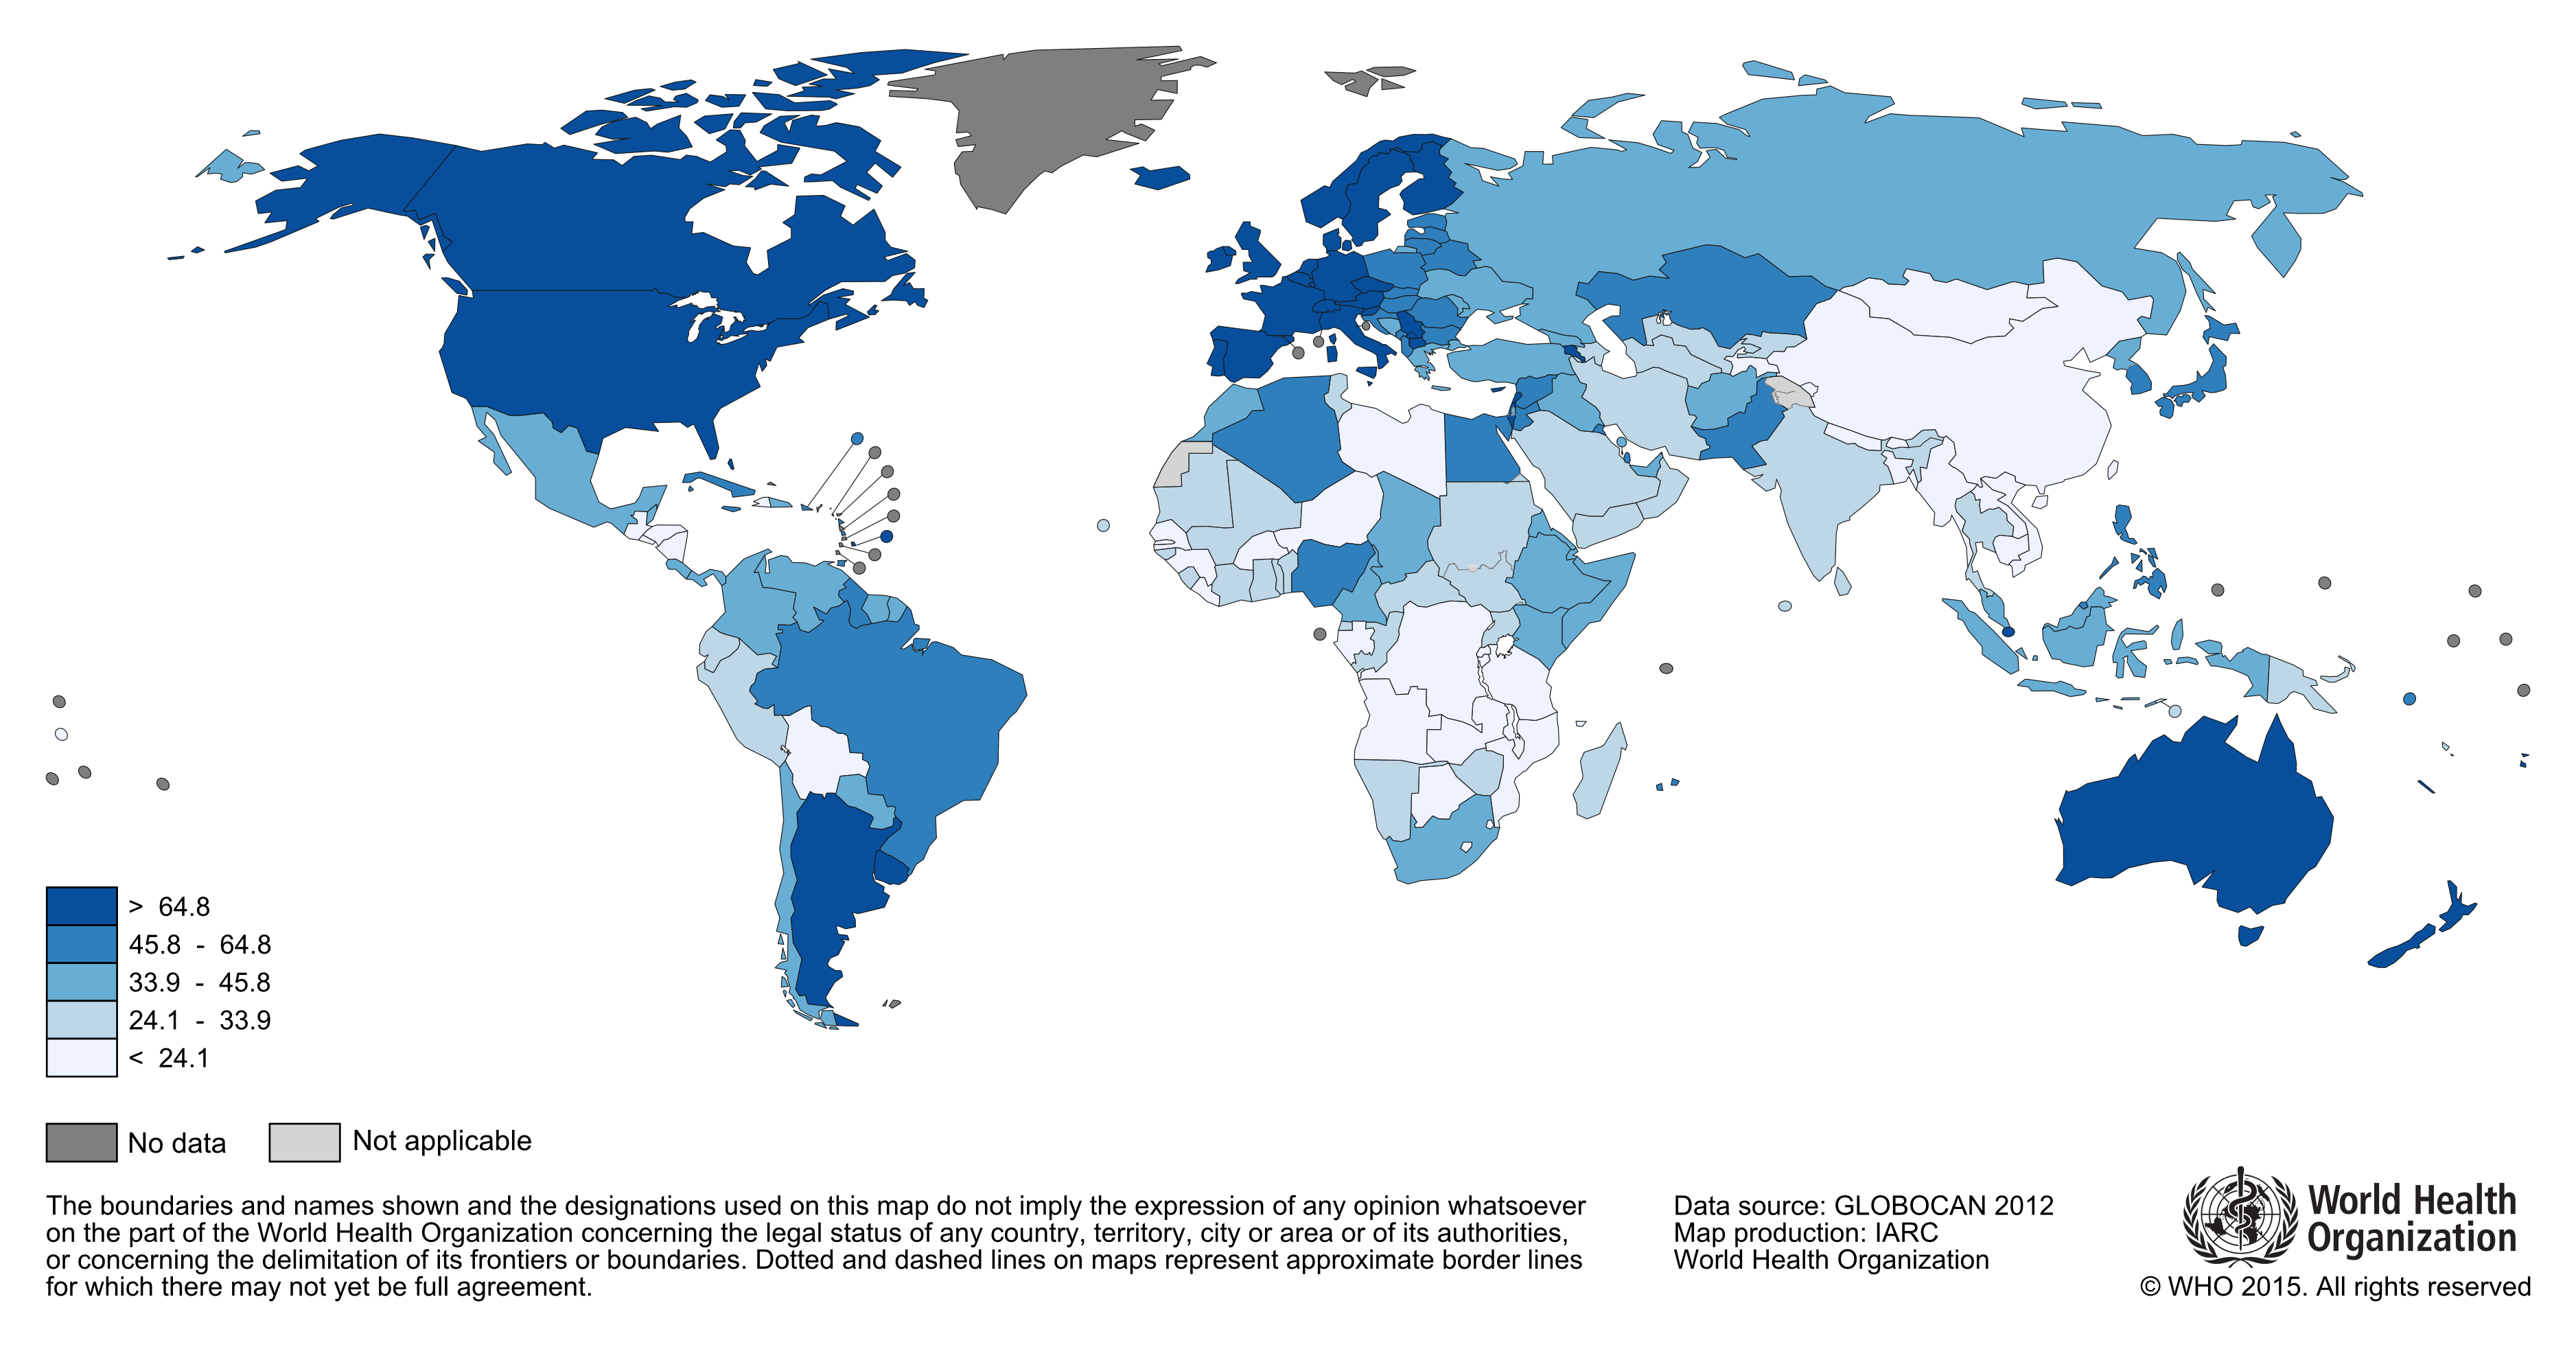
\includegraphics[width=1\textwidth]{imagenes/breast_map.png}
\end{figure}
\end{frame}

\end{comment}


%
%\begin{frame}{Histological Grading}
%\begin{itemize}
%\item<1-> The suspicious tissue is analyzed after a hematoxylin and eosin histological procedure
%\item<2->  Bloom and Richardson modified grading system is recommended by WHO
%\end{itemize}
%\begin{figure}
%\includegraphics<1>[width=1\linewidth]{imagenes/biopsia.png}
%\end{figure}
%\vspace{-1cm}
%\begin{figure}
%\hspace{-5cm}\includegraphics<2-3>[height=0.55\textheight]{imagenes/biopsia1.png}
%\includegraphics<4>[height=0.55\textheight]{imagenes/biopsia2.png}
%\includegraphics<5->[height=0.55\textheight]{imagenes/biopsia3.png}
%\end{figure}
% \begin{textblock}{10}(7,7.5)
% \begin{itemize}
% \item<3-> \textcolor{UniRed}{\textbf{Nuclear Pleomorphism Scoring}}
% \end{itemize}
% \end{textblock}
% \begin{textblock}{10}(7,10)
% \begin{itemize}
% \item<4-> Tubule Count
% \end{itemize}
% \end{textblock}
% \begin{textblock}{10}(7,13)
% \begin{itemize}
% \item<5-> Mitotic Count
% \end{itemize}
% \end{textblock}
%% \item\tiny Nuclear Pleomorphism Scoring 
%% \item\tiny Tubule Count
%% \item\tiny Mitotic Activity
%
%
%
%\end{frame}
%
%
%\begin{frame}{pleomorphism}
%\frametitle{Breast Cancer}
%\framesubtitle{Nuclear pleomorphism (NP)}
%\begin{columns}[t, totalwidth=1\textwidth]
%\begin{column}{0.55\linewidth}
%\begin{itemize}\justifying 
%\item<1-> NP refers to variations in nucleus size and shape.
%\item<2-> Agreement is reported to be $0.3<\kappa<0.5$ ($0<\kappa<1$)\footnote{\tiny{Meyer JS, et al. Breast carcinoma malignancy grading by Bloom-Richardson system vs proliferation index: reproducibility of grade and advantages of proliferation index. Mod Pathol. 2005}}
%\item<3-> \normalsize{Grading is improved when the nuclei size is known}\footnote{\tiny{Veta M, et al. Prognostic value of automatically extracted nuclear morphometric features in whole slide images of male breast cancer. Mod Pathol. 2012}}
%\footnote{\tiny{Prvulović I et. al. Morphometry of tumor cells in different grades and types of breast cancer. Coll Antropol. 2010\\}}
%\end{itemize}
%\end{column}
%\begin{column}{0.4\linewidth}
%\begin{figure}
%\includegraphics<1->[width=\textwidth]{imagenes/lupita.jpg}
%\end{figure}
%\end{column}
%\end{columns}
%\end{frame}
%
%
%
%\begin{frame}
%%\frametitle{Motivation}
%\frametitle{Qualitative Estimation}
%\begin{columns}[t, totalwidth=1\textwidth]
%\begin{column}{0.65\linewidth}
%\begin{figure}\includegraphics<1-2>[width=1\linewidth]{imagenes/pleomofinal11.jpg}
%\includegraphics<3-4>[width=1\linewidth]{imagenes/pleomofinal12.jpg}
%\includegraphics<5-6>[width=1\linewidth]{imagenes/pleomofinal13.jpg}
%\end{figure}
%\end{column}
%\begin{column}{0.34\linewidth}
%\parskip 5pt
%\par {NP score 1:}
%\footnotesize 
%\begin{itemize}[topsep=2pt]
%\item<1-> Little variation in size 
%\item<2->  Regular outlines
%\end{itemize}
%\parskip 5pt
%\par \uncover<3->{NP score 2:}
%\begin{itemize}[topsep=2pt]
%\item<3->  Moderate variability in size and shape
% \item<4->  Visible nucleoli 
%\end{itemize}
%\parskip 5pt 
%\par\uncover<5->{NP score 3:}
%\begin{itemize}[topsep=2pt]
%\item<5->  Marked variation in size and shape 
%\item<6->  Prominent nucleoli
%%\item Very large and bizarre forms
%\end{itemize}
%\end{column}
%\end{columns}
%\end{frame}
%
%
%
%\begin{frame}
%\frametitle{Nuclear Pleomorphism in the practice}
%\LARGE \begin{block}{}
%\justifying NP gives an evaluation of the aggressiveness of the tumour and has correlation with biological variables (bio-marker)\footnote{\tiny{Abdalla F et al., Correlation of nuclear morphometry of breast cancer in histological sections with clinicopathological features and prognosis. Anticancer Res. 2009 }}\footnote{\tiny{Yang Q et al., Correlation between nuclear grade and biological prognostic variables in invasive Breast Cancer 2001\\}}
%\end{block}
%\end{frame}




\begin{frame}{First Aproach}
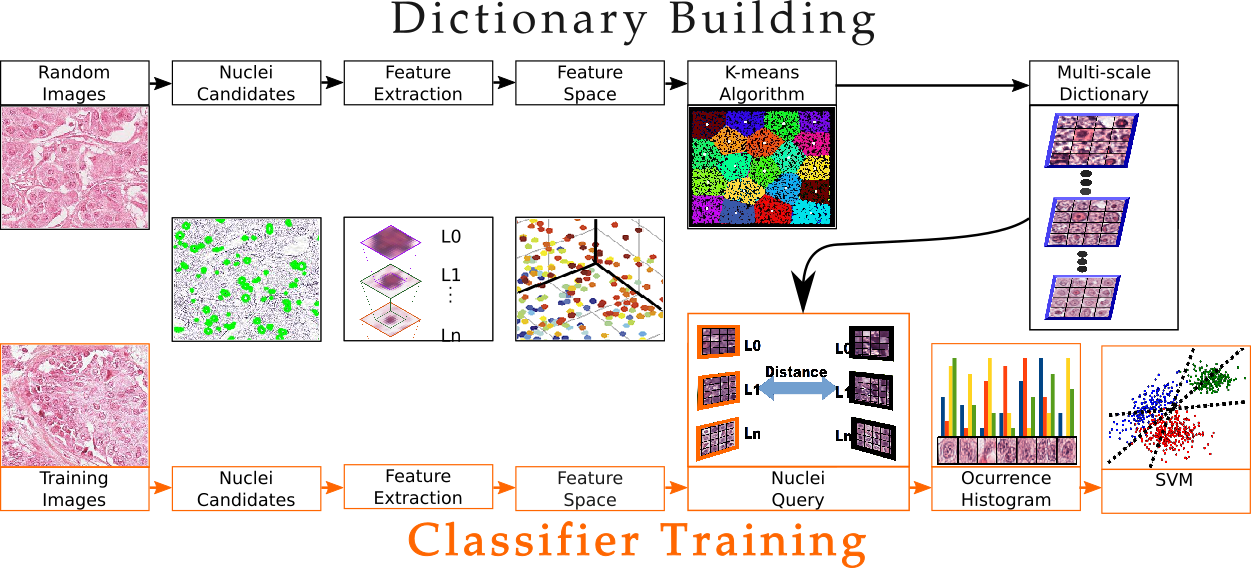
\includegraphics[width=\textwidth]{imagenes/metodo_BoF.png}
\end{frame}



\begin{comment}
\begin{frame}{Problem}
\frametitle<presentation>{Problem}
% In the nuclear pleomorphism a quantitative and qualitative judgment is made and
% problems of consistency and reproducibility are found. Morphological features
% could give a correlation with clinicopathological features and prognosis.

\LARGE \begin{block}{}
A quantitative measurement of nuclear pleomorphism is not currently available %because it is difficult to implement in the routine diagnostic workflow.


\end{block}

\end{frame}%
\end{comment}
% The following outlook is optional.



%\section{NP Quantification Strategy}


\begin{frame}{Nuclei Detection}
%\hspace*{-3cm}
\begin{itemize}
\item<1-> \small Using a color deconvolution technique the Hematoxylin (H) and eosin (E) stains are estimated% \footnote{\tiny{A method for normalizing histology slides for quantitative analysis, Macenko et al.ISBI 2009}}
\item<3-> \small Watershed algorithm is used to detect nuclei candidates in H stain%\footnote{\tiny{Veta M.,ISBI 2011}}
\item<4-> \small Final candidates are found after morphological operations
\end{itemize}

\begin{textblock*}{2cm}(1cm,6cm) % {block width} (coords)
\begin{figure}
\includegraphics<1->[width=2cm]{MSER/1.jpeg}
\end{figure}
\end{textblock*}
\begin{textblock*}{2cm}(3.2cm,6cm) % {block width} (coords)
\begin{figure}
\includegraphics<2->[width=2cm]{MSER/2.jpeg}
\end{figure}
\end{textblock*}
\begin{textblock*}{2cm}(5.4cm,6cm) % {block width} (coords)
\begin{figure}
\includegraphics<3->[width=2cm]{MSER/3.jpeg}
\end{figure}
\end{textblock*}
\begin{textblock*}{2cm}(7.6cm,6cm) % {block width} (coords)
\begin{figure}
\includegraphics<4->[width=2cm]{MSER/4.jpeg}
\end{figure}
\end{textblock*}
\begin{textblock*}{2cm}(9.8cm,6cm) % {block width} (coords)
\begin{figure}
\includegraphics<5->[width=2cm]{MSER/5.jpeg}
\end{figure}
\end{textblock*}
\end{frame}

\begin{frame}{Multi-scale Feature Extractor}
\begin{itemize}
\item<1->\justifying The characterization of each nucleus candidate was performed by analyzing multiple scales 
\item<2-> \justifying The feature vector corresponds to the information from RGB patches which are concatenated along one dimension.
\end{itemize}
\begin{figure}
\hspace{-1cm}\includegraphics<1->[width=7cm]{imagenes/descriptor.jpg}
\end{figure}
 \begin{textblock}{20}(11,10)
  \onslide<2->{$F(X_i)=\lbrace L0,L1,L2\rbrace$}
 \end{textblock}
\end{frame}

\begin{frame}{Results  F1-Score}

The F-score is used to evaluate the classification
\begin{equation}
    F_{\beta} = (1+\beta^{2}).\frac{precision.recall}{(\beta^{2}.precision)+recall}
\end{equation}
$\beta=1$ is used this is the harmonic mean between precision and recall
\end{frame}

\begin{frame}{Dataset - Mitos Atypia 14}

\begin{table}[]
\begin{tabular}{|c|c|}
\hline
\centering
Grade &  \#40X images \\ \hline
NP 1  & 92    \\ \hline
NP 2  & 900  \\ \hline
NP 3  & 208    \\ \hline
\end{tabular}
\caption{Training and validation - 11 cases for training}
\end{table}
\begin{table}[]
\begin{tabular}{|c|c|}
\hline
Grade & \# 40X images \\ \hline
NP 1  & 152           \\ \hline
NP 2  & 252           \\ \hline
NP 3  & 92            \\ \hline
\end{tabular}
\caption{Test dataset - 5 cases}
\end{table}
    
\end{frame}


\begin{frame}{Results}
\begin{table}[]
\begin{tabular}{|c|c|c|}
\hline
Experiment/S.Patch & \begin{tabular}[c]{@{}c@{}}32x32\\ L2\end{tabular} & \begin{tabular}[c]{@{}c@{}}20x20\\ L2\end{tabular} \\ \hline
1 vs 2 and 3       & \textbf{0.593}                                              & 0.434                                              \\ \hline
3 vs 1 and 2       & \textbf{0.642}                                              & 0.47                                               \\ \hline
1 vs 2             & \textbf{0.7128}                                             & 0.47                                               \\ \hline
1 vs 3             & 0.660                                              & \textbf{0.7029}                                             \\ \hline
2 vs 3             & \textbf{0.6759}                                             & 0.5813                                             \\ \hline
\end{tabular}
\caption{Results Bag Of Features}
\end{table}
\end{frame}

\begin{frame}{Current Work}

\begin{itemize}
    \item \textbf{To enhance the automatic nuclear pleomorphism grading}
    \item To find out if there is a relationship between the nuclear grade quantification with the cancer recurrence
\end{itemize}
    
\end{frame}


\begin{frame}{CNN Framework}
    \centering
    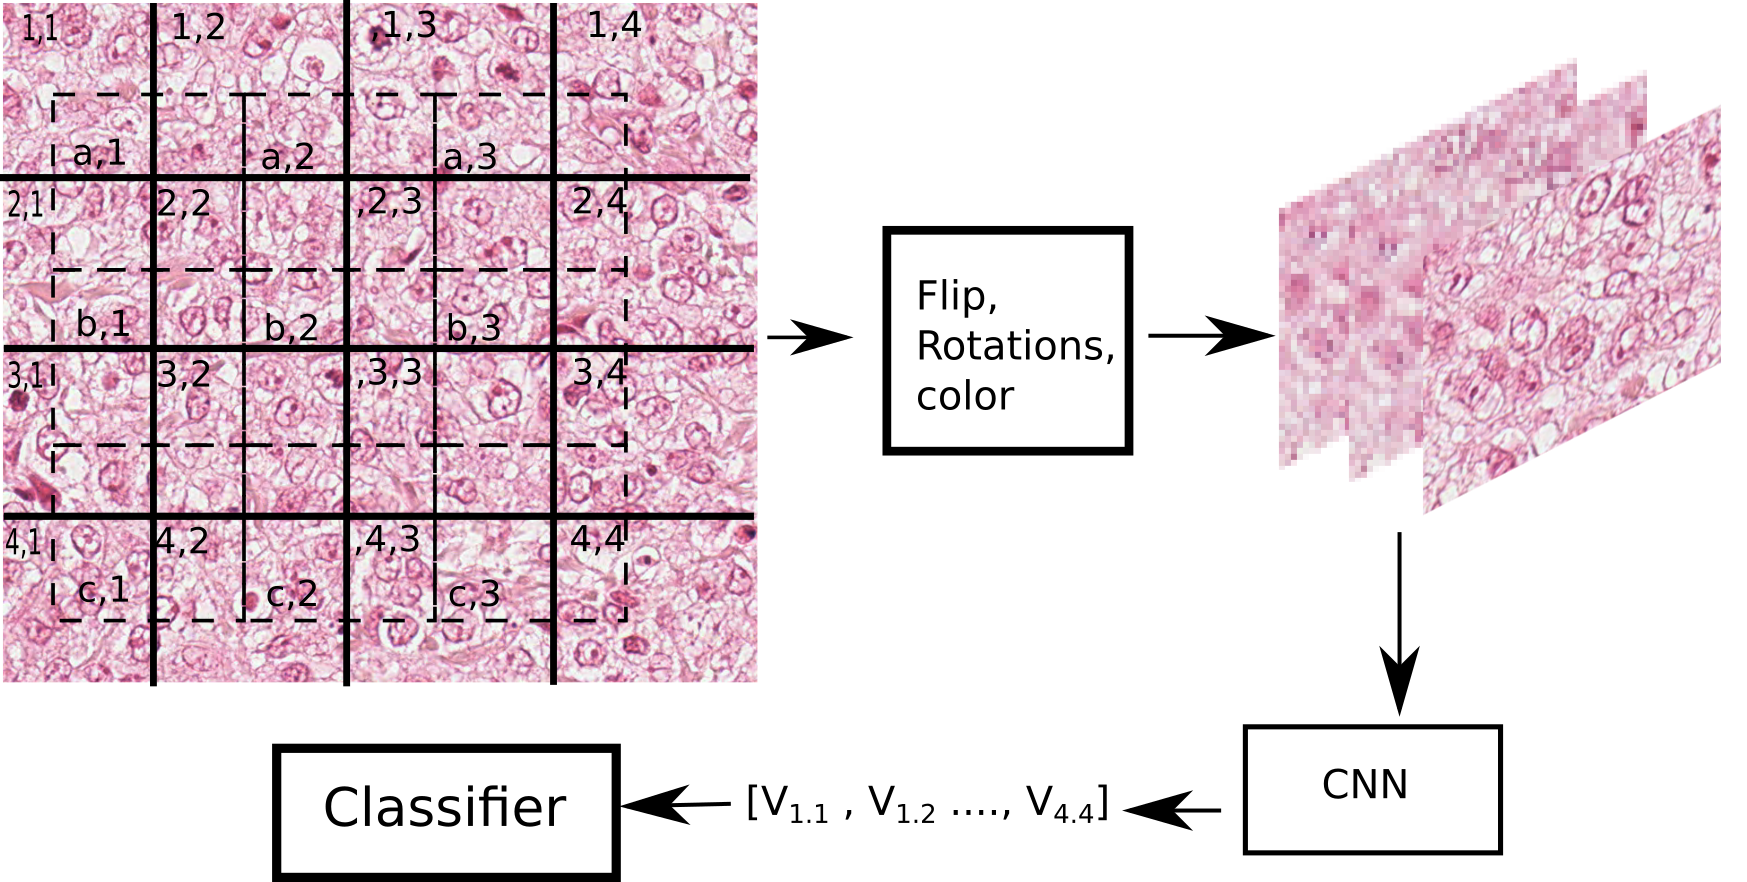
\includegraphics[width=1\textwidth]{imagenes_cnn/CCn_methodF.png}
 
\end{frame}

\begin{frame}{CNN Framework}
    \centering
   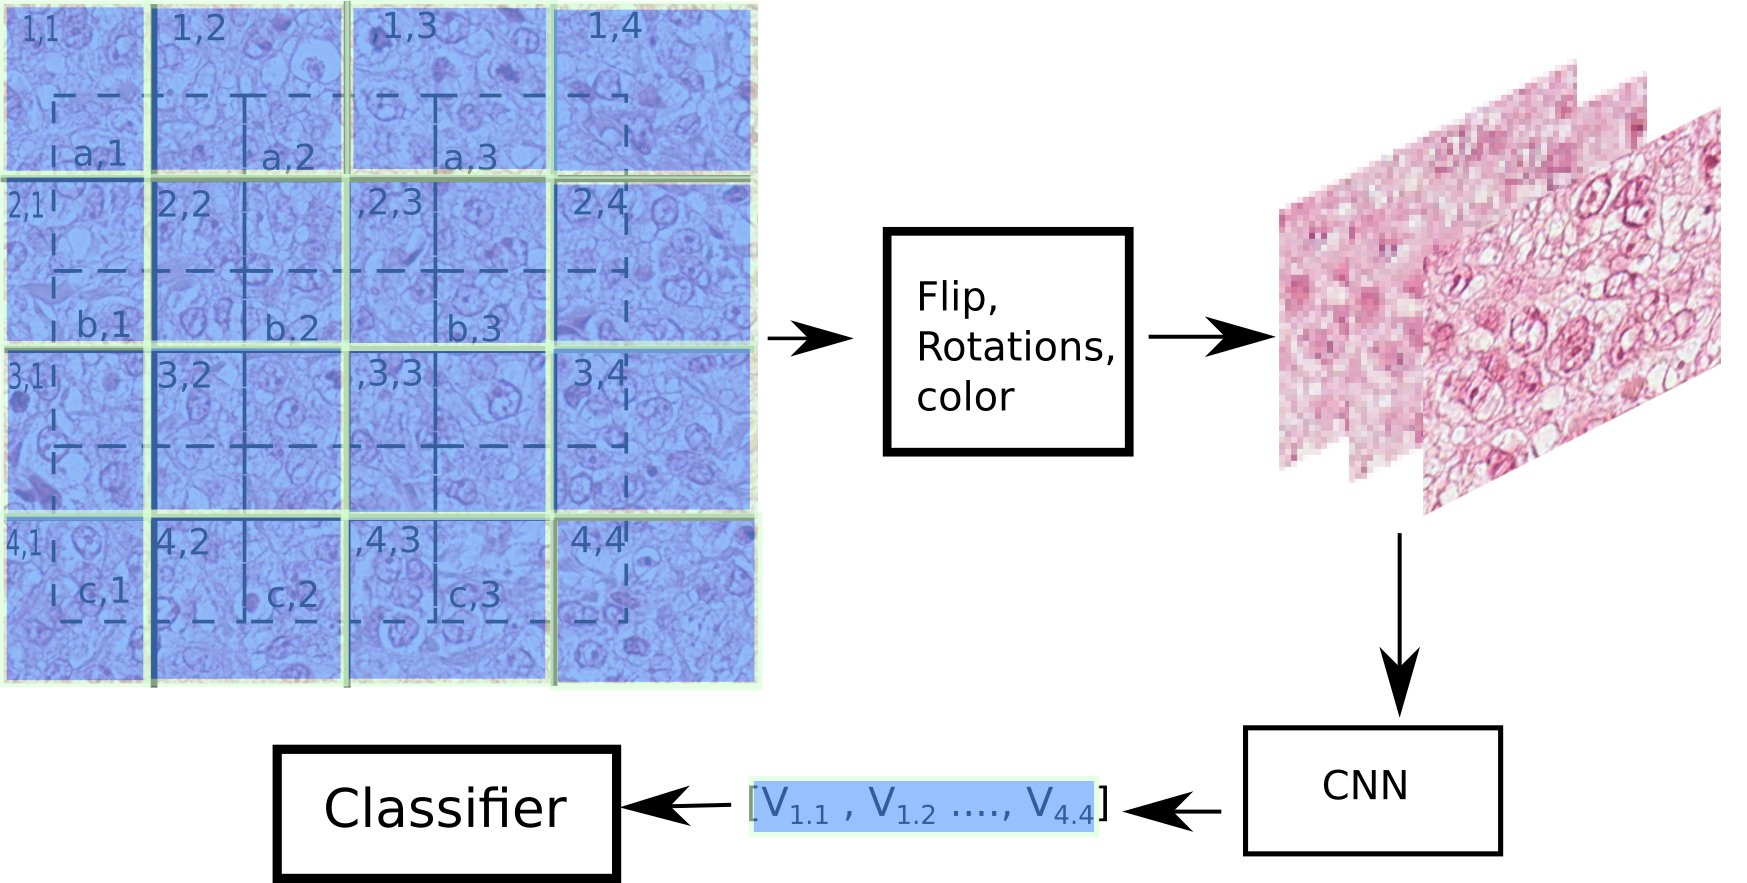
\includegraphics[width=1\textwidth]{imagenes_cnn/CCn_methodFS2.png}
\end{frame}




\begin{frame}{Dataset- Mitos Atypia 14}

\begin{table}[]
\begin{tabular}{|m{1cm}|m{2cm}|m{3cm}|m{1.3cm}|m{1.3cm}|}
\hline
\centering
Grade &\centering  \#40X images &\centering Total Patches 344x344 pixels&\centering  Train & Validation \\ \hline
NP 1  & 92            & 21,344  &   18,144   & 3,200          \\ \hline
NP 2  & 900           & 22,500  &  19,096    & 3,404     \\ \hline
NP 3  & 208           & 20,800  &  17,764    & 3,036     \\ \hline
\end{tabular}
\caption{Training and validation - 11 cases for training}
\end{table}
    \begin{table}[]
\begin{tabular}{|c|c|}
\hline
Grade & \# 40X images \\ \hline
NP 1  & 152           \\ \hline
NP 2  & 252           \\ \hline
NP 3  & 92            \\ \hline
\end{tabular}
\caption{Test dataset - 5 cases}
\end{table}
\end{frame}


\begin{frame}{Results}
\begin{table}[]
\begin{tabular}{|p{1.5cm}|p{1.4cm}|p{1.3cm}|p{1.3cm}|p{1.3cm}|p{1.3cm}|}
\hline
              & CNN (1024dim)  & CNN (3dim)     & VGG16 & Alexnet & Resnet50       \\ \hline
3Vs.1 and 2 & 0.635          & 0.523          & 0.629 & 0.493  & \textbf{0.685} \\ \hline
1Vs.2 and 3 & \textbf{0.676} & 0.645          & 0.564 & 0.581  & 0.573          \\ \hline
1 Vs 2        & 0.637         & \textbf{0.664} & 0.453 & 0.623   & 0.592         \\ \hline
2 Vs 3        & 0.570          & 0.567          & 0.544 & 0.619   & \textbf{0.670} \\ \hline
1 Vs 3        & 0.666         & \textbf{0.672} & 0.620 & 0.649   & 0.563          \\ \hline
\end{tabular}
\end{table}    



\end{frame}



\begin{comment}
\begin{frame}{Results}

\begin{table}[]
\begin{tabular}{|l|l|l|l|}
\hline
Experiment  & Validation  & test patches & FOV on test \\ \hline
CNN 1       & 0.78           & 0.266                & 0.482                          \\ \hline
CNN 2       & 0.8345         & 0.290                & 0.53                           \\ \hline
Fully CNN   & 0.3481         &                      &                                \\ \hline
Khan et al. & 0.845(k-fold)          &                      & \textbf{0.71}*                  \\ \hline
BoF         &                &                      & 0.66 *                          \\ \hline
\end{tabular}
\caption{Accuracy - * 11 cases for train, 5 for test}
\end{table}
\end{frame}



\end{comment}

%
%\begin{frame}{}
%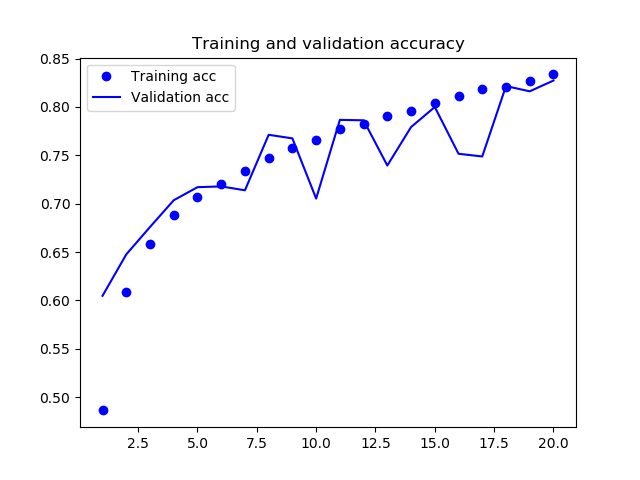
\includegraphics[width=\textwidth]{imagenes/ResultACCepoch.png}
%    
%\end{frame}

%\begin{frame}{Confusion Matrix}
%
%\begin{table}[]
%\begin{tabular}{|c|c|c|}
%\hline
%51 & 97  & 4  \\ \hline
%17 & 195 & 40 \\ \hline
%5  & 67  & 20 \\ \hline
%\end{tabular}
%\caption{for CNN2}
%\end{table}
%    
%\end{frame}


\begin{frame}{Spatial Pyramidal Characterization }

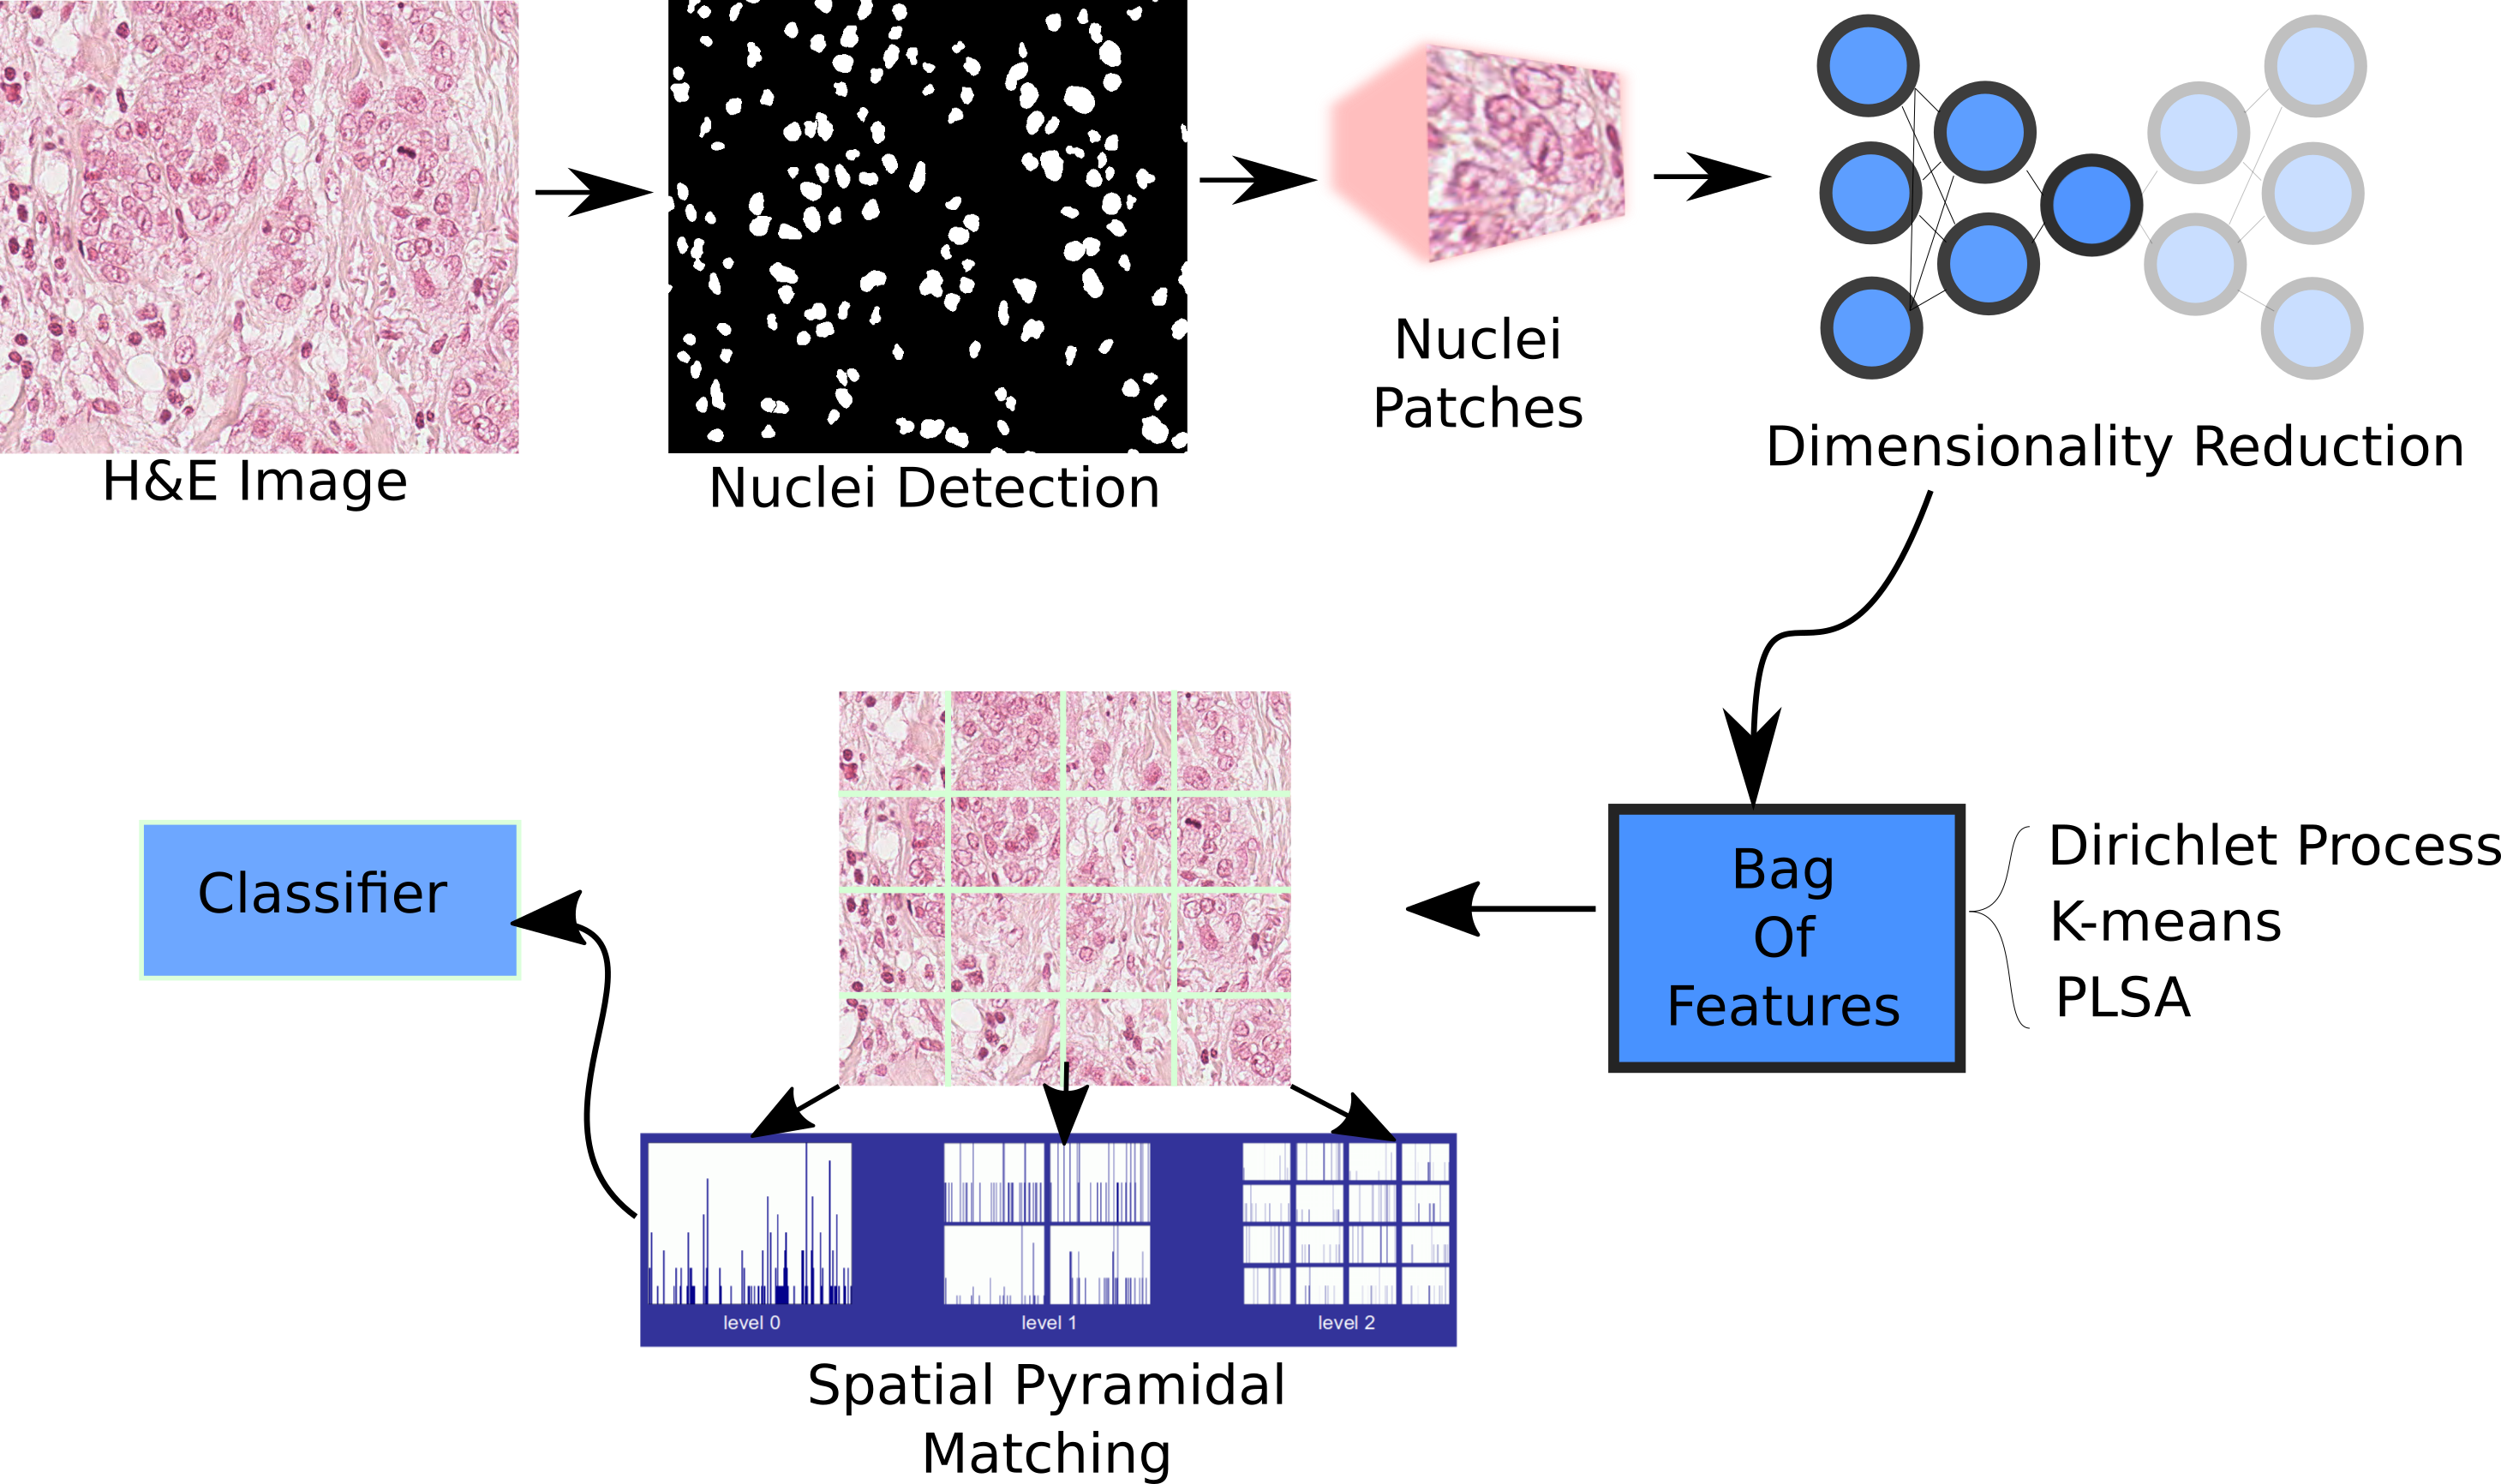
\includegraphics[width=\textwidth]{imagenes_cnn/metodonuevo.png}
    
\end{frame}



\begin{frame}{Nuclei Detection}

\begin{itemize}
    \item Color deconvolution to find hematoxylin channel (Macenko et al.)
    \item Watershed Algorithm to find connected components at different scales (Veta et al.)
    \item Patches are extracted using the nuclei centroid as seed (72x72 pixels)
\end{itemize}
    
\end{frame}

\begin{frame}{Dimensionality Reduction- Convolutional autoencoder}
\begin{itemize}
    \item 3 convolutional layer for encoding and 3 for decoding
    \item 2048 dimensions in coded representation for nuclei (22.5 compresion factor)
    \item 6300 dim feature vector ({LO,L1,L2})
\end{itemize}
    \centering
    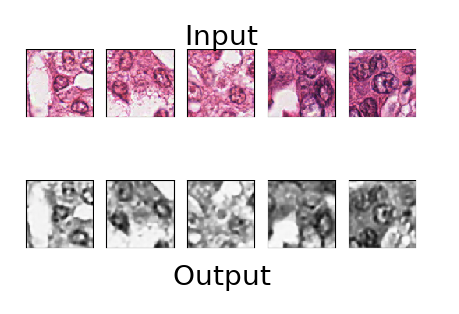
\includegraphics[width=0.65\textwidth]{imagenes_cnn/autoencoderresponse.png}
    \\Autoncoder Reconstruction
\end{frame}




\begin{frame}{Results}

\begin{table}[l]
\begin{tabular}{|m{1.2cm}|m{1cm}|m{1cm}|m{1cm}|m{1cm}||m{1cm}|m{1cm}|m{1cm}|}
\hline
              & PS.  & PS L0   & PS L01 & PS L2 & BOF PY          & BOF PY L0       & BOF PY L1\\ \hline
3 Vs. 1 and 2 & 0.578     & \textbf{0.630} & 0.565        & 0.53         & 0.624          & 0.593           & 0.583\\ \hline
1 Vs. 2 and 3 & 0.624    & 0.564          & 0.520         & 0.489        & \textbf{0.692} & 0.642           & 0.678\\ \hline
1 Vs 2        & 0.473     & 0.597          & 0.542         & 0.573        & 0.650           & \textbf{0.713} & 0.660\\ \hline
2 Vs 3        & 0.560     & 0.603          & 0.606         & 0.632        & 0.722          & 0.660           & \textbf{0.729}\\ \hline
1 Vs 3        & 0.623     & 0.716          & 0.639         & 0.632       & 0.628          & 0.675         & \textbf{0.740} \\ \hline
\end{tabular}
\end{table}
    
\end{frame}



\begin{frame}{New Dataset}
    \begin{table}[]
\begin{tabular}{|c|c|}
\hline
Grading              & \# Marked Areas \\ \hline
Grade 1              & 135             \\ \hline
Grade 2              & 132             \\ \hline
Grade 3              & 39              \\ \hline\hline
\textbf{Total Cases} & \textbf{24}     \\ \hline
\end{tabular}
\end{table}
\end{frame}



\begin{frame}{Final Remarks}

\begin{itemize}
    \item The Slightly variation between the NP grades and the high tissue variability makes difficult to find an adequate model.
    \item The CNN model could be improved if take advantage of the spatial information
    \item The auto-encoder representation and vocabulary construction maybe is not the most appropriate.
\end{itemize}
    
\end{frame}








\begin{frame}
    Thank you...
\end{frame}





\begin{frame}
  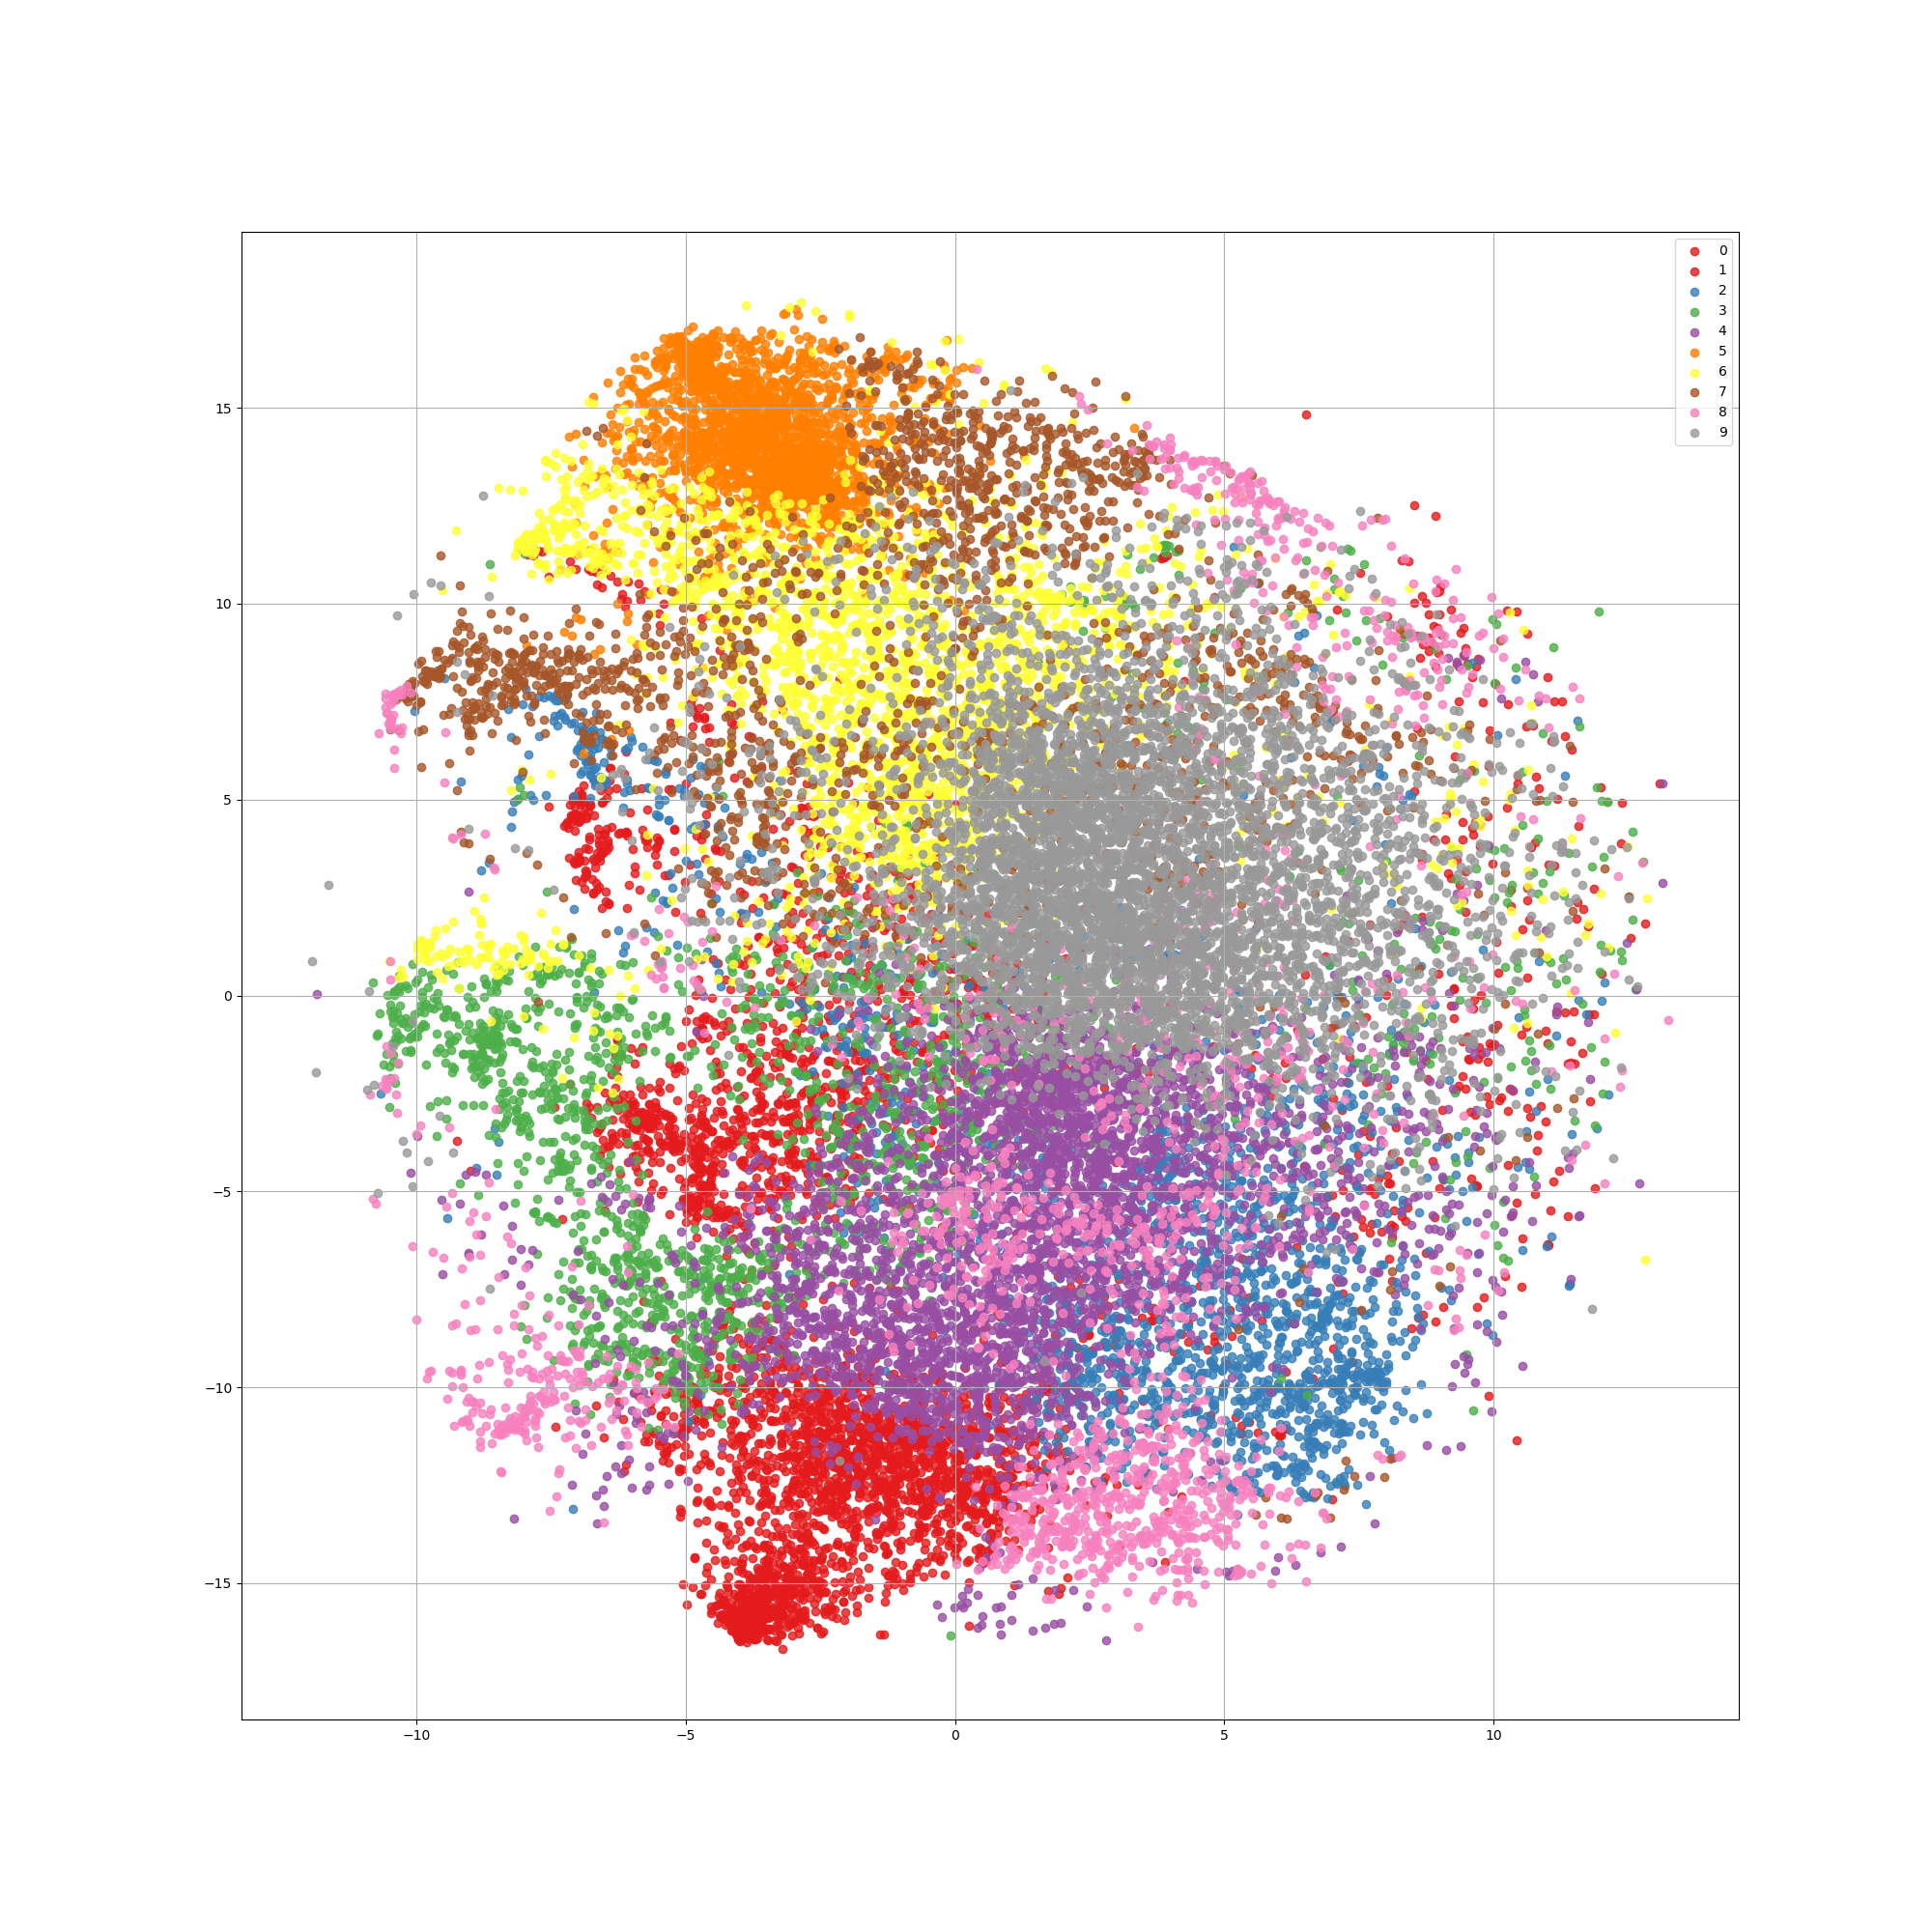
\includegraphics[width=\textwidth]{imagenes_cnn/Tsne_alpha90_cluster10.png}
\end{frame}



%\begin{frame}{Visual Results - multiscale and cosine transform}
%\centering
%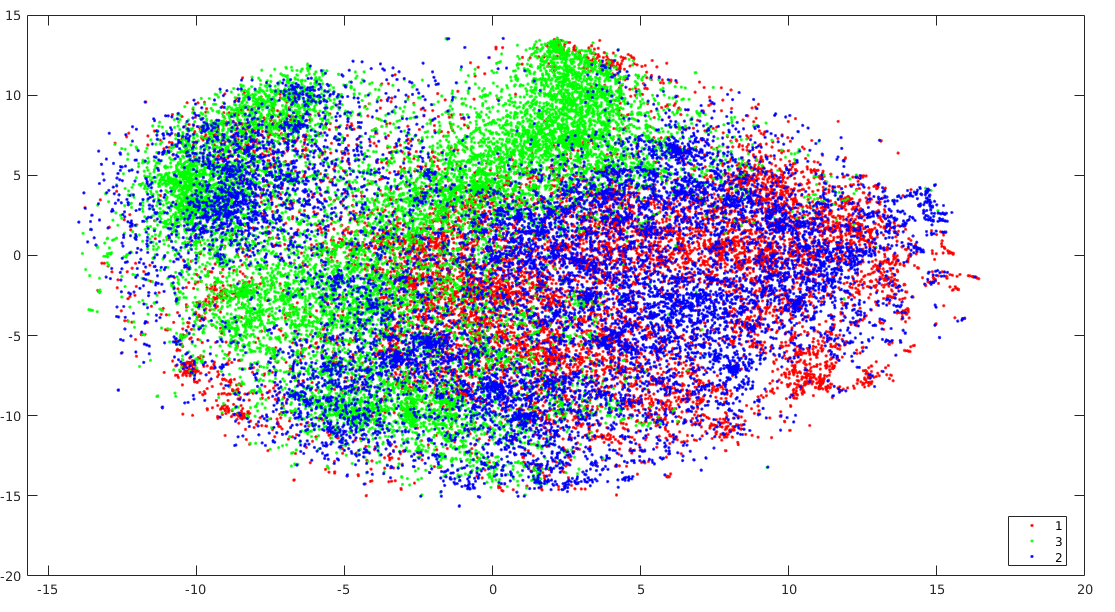
\includegraphics[width=0.85\textwidth]{imagenes/all.png}
%\end{frame}

%\begin{frame}{Visual Results - Space by topic}
%\vspace{-0.45cm}
%\begin{table}[]
%\begin{tabular}{ll}
% 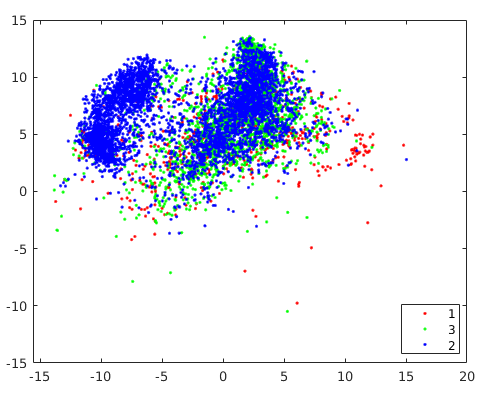
\includegraphics[width=0.31\textwidth]{imagenes/cluster3.png}& 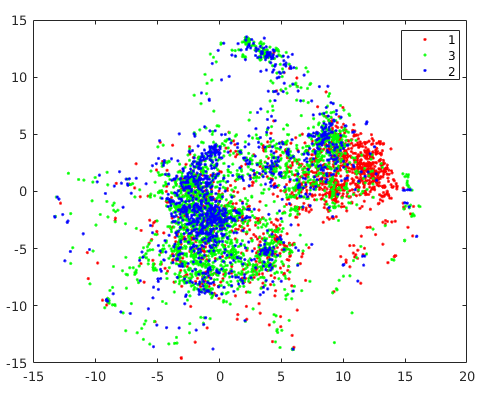
\includegraphics[width=0.31\textwidth]{imagenes/cluster4.png} \\
%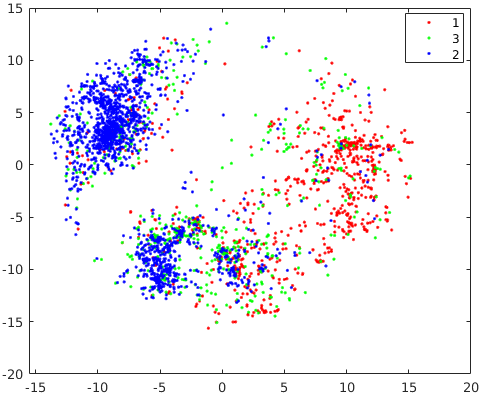
\includegraphics[width=0.31\textwidth]{imagenes/cluster8.png} & 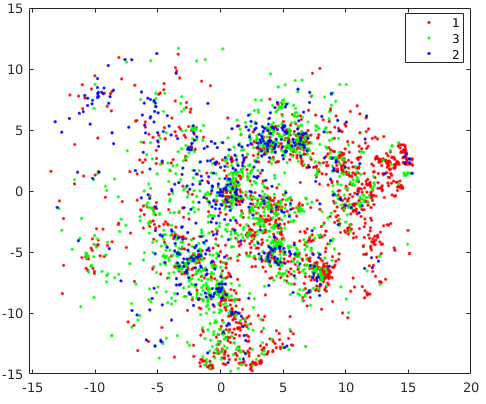
\includegraphics[width=0.31\textwidth]{imagenes/clustes7.png}
%\end{tabular}
%\end{table}
%
%\end{frame}


\begin{frame}{Proposed Grading Methodology}
\begin{figure}
\centering
\includegraphics<1>[width=0.95\linewidth]{imagenes/metodo_sipaim2017.png}
\end{figure}
\end{frame}



%
%
%\begin{frame}{Bag of Features Construction}
%\begin{columns}
%\begin{column}{4cm}
%\begin{overprint}
%\begin{figure}
%\includegraphics<1>[width=0.95\textwidth]{dicc/kmeans.png}
%\includegraphics<2>[width=0.95\textwidth]{dicc/1.png}
%\includegraphics<3>[width=0.95\textwidth]{dicc/2.png}
%\includegraphics<4>[width=0.95\textwidth]{dicc/3.png}
%\includegraphics<5>[width=0.95\textwidth]{imagenes/unehistogram.png}
%\includegraphics<6>[width=0.95\textwidth]{imagenes/multiplehistogram.png}
%\caption{\only<1>{K-means Algorithm}\only<2>{Dictionary with L0}\only<3>{Dictionary with L1}
%\only<4>{Dictionary with L2}\only<5>{Occurrence histogram for one image}\only<6>{Occurrence histogram for Train images}}
%\end{figure}
%\end{overprint}
%%\vspace{0.5cm} 
%\end{column}
%\begin{column}{8cm}
%\begin{overprint}
%\begin{itemize}
%\item<1-> The multi-scale feature space is  partitioned with a $k$-medoids algorithm
%\item <2->Each medoid correspond to a visual word in the BoF
%\item<5-> Each new candidate from a train or test image is represented by some atom in the dictionary, using a cosine distance to find the nearest.
%\end{itemize}
%\end{overprint}
%\end{column}
%\end{columns}
%\end{frame}
%
%\begin{frame}{Associated BoF Graph Construction}
%\begin{itemize}
%\item\small The complete set of high dimensional features are reduced to 2D space using t-distributed stochastic neighbor embedding (t-SNE)
%\pause
%\item\small The 2D space built preserve the high dimensional data structure
%\pause
%\item\small The visual-words from the BoF are projected to the 2D space and a nearest graph is build
%\end{itemize}
%\begin{figure}
%\includegraphics<1-2>[width=0.93\textwidth]{imagenes/proyeccion2D.png}
%\includegraphics<3>[width=0.93\textwidth]{imagenes/proyeccion2Dgrafo.png}
%\includegraphics<4->[width=0.93\textwidth]{imagenes/grafo_midx.png}
%
%\end{figure}
%\end{frame}
%
%
%\begin{frame}{Filtering Signal on Graph}
%\begin{itemize}
%%\item<1-> The notion of frequency in the graph is possibly by using the Laplacian graph operator \textcolor{red}{referencia}
%\item<1-> The histogram from the BoF is used as signal on the built graph
%\item<2-> A filtering operation is performed to spread the signal over the graph  \
%\end{itemize}
%\begin{columns}          
%  \begin{column}{5cm}     
%	\begin{figure}
%		\includegraphics<2-> [height=3.5cm]{imagenes/senal1.png}
%        \onslide<2->{\caption {Histogram over Graph}}
%	\end{figure}
%	\end{column}
%\begin{column}{5cm}    
%	\begin{figure}
%\includegraphics<3-> [height=3.5cm]{imagenes/senal_filtrada1.png}
%	\onslide<3->{\caption{Filtered signal on Graph}}
%		
%	\end{figure}
%\end{column}           
%    \end{columns}
%
%
%\end{frame}
%
%\begin{frame}{Updated Histogram}
%\begin{itemize}
%\item<1->The resulting signal after the filtering operation is used as an updated histogram were the neighbor relationships are preserve
%\item<2-> The updated histogram is used as fed in a SVM
%\end{itemize}
%\begin{columns}          
%  \begin{column}{5cm}     
%	\begin{figure}
%		\includegraphics<1-> [width=0.97\textwidth]{imagenes/histogram1.png}\caption {Previous histogram}
%	\end{figure}
%	\end{column}
%\begin{column}{5cm}    
%	\begin{figure}
%	\only<2>{\includegraphics<2> [width=0.97\textwidth]{imagenes/histogram_filt1.png}
%	\caption{\only<2>{New histogram}}
%	}
%		
%	\end{figure}
%\end{column}           
%    \end{columns}
%\end{frame}
%
%\section{Experiments and Results}
%
%\begin{frame}
%
%\frametitle{Experiments and Results}
%\framesubtitle{BCa Dataset}
%\centering
%\footnotesize \begin{block}{The Carcinoma Atlas (TCGA)}
%\begin{itemize}
%\item 14 Breast cancer histological samples (134 FoVs)
%\item FoVs selected by an expert from the Department of Pathology, Universidad Nacional.
%\end{itemize}
%\end{block}
%\begin{figure}
%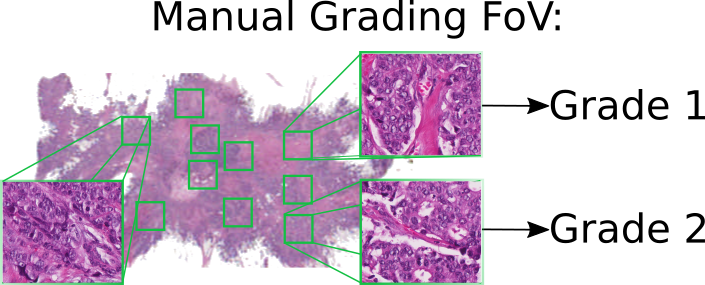
\includegraphics[width=6.5cm]{imagenes/fov.png}
%\end{figure}
%\end{frame}
%
%\begin{frame}{Experimental Setup}
%\footnotesize\begin{itemize}
%\item The window sizes were: $4\times4$, $8\times8$, $12\times12$ and $16\times16$
%\pause
%\item The number of layers for each window was: $1$, $2$ and $3$
%\pause
%\item The number of Visual words: $1600$ and $6000$ 
%\pause
%\item The associated BOF graph was built using $60$ neighbors for each node
%\pause
%\item The filter aplied in the graph:  (a) Half cosine filter   and (b) a first order low pass filter (only one)
%\end{itemize}
%\vspace{-1cm}
%\begin{columns}[t, totalwidth=1\textwidth]
%\begin{column}{0.5\textwidth}
%\begin{figure}
%\includegraphics<5->[width=0.9\textwidth]{imagenes/cosine_filter.png}
%\end{figure}
%\vspace{-0.5cm}\centering\small\onslide<5->{Half-cosine Filter}
%\end{column}
%\begin{column}{0.5\textwidth}        
%\begin{figure}
%\includegraphics<6->[width=0.9\textwidth]{imagenes/lowpass_filter.png}
%\end{figure}
%\vspace{-0.5cm}\centering\small\onslide<6->{Lowpass Filter}
%\end{column}        
%\end{columns}
%\end{frame}
%
%
%\begin{frame}{Methods for comprarision}
%\begin{block}{Two Baselines were used:}
%\begin{enumerate}
%\item BoF only Approach
%\item Morphometric measurement as feature vector (Area, perimeter, round factor)
%\end{enumerate}
%\end{block}
%\end{frame}
%
%\begin{frame}{Results}
%\framesubtitle{Qualitative Results}
%\begin{itemize}
%\item In the figures, some nuclei candidates (left) and their corresponding representation in the dictionary (right) are shown
%\end{itemize}
%\vspace{-0.8cm}
%\begin{columns}[t, totalwidth=1\textwidth]
%\begin{column}{0.5\textwidth}
%\begin{center}
%\begin{figure}
%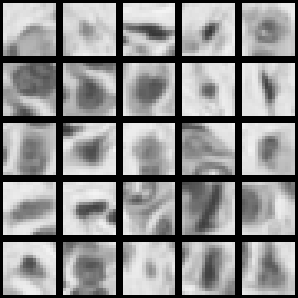
\includegraphics[width=0.9\textwidth]{imagenes/nuclei_test.png}
%\end{figure}
%\centering\small Test Image
%\end{center}
%\end{column}
%\begin{column}{0.5\textwidth}         % \begin{block}
%\begin{center}
%\begin{figure}
%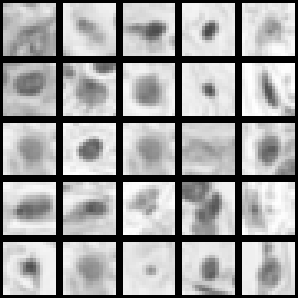
\includegraphics[width=0.9\textwidth]{imagenes/diccionario_test.png}
%\end{figure}
%\centering\small BoF Representation
%\end{center} 
%\end{column}
%\end{columns}
%\end{frame}
%
%
%\begin{frame}{Results}
%\framesubtitle{Qualitative Results}
%\begin{itemize}
%\item Nuclei Representation in the associated graph
%\end{itemize}
%\begin{figure}
%\includegraphics<1>[width=0.85\textwidth]{imagenes/grafo1a.png}
%\includegraphics<2>[width=0.85\textwidth]{imagenes/grafo2a.png}
%\includegraphics<3>[width=0.85\textwidth]{imagenes/grafo3a.png}
%\end{figure}
%
%\small\centering
%\onslide<1>{Medoids from Images NP score 1}
%\small\centering
%\onslide<2>{Medoids from Images NP score 2}
%\small\centering
%\onslide<3>{Medoids from Images NP score 3}
%\end{frame}
%
%\begin{frame}{Quantitative Results}
%\begin{columns}[t, totalwidth=1\textwidth]
%\begin{column}{0.5\textwidth}
%\begin{center}
%\begin{figure}
%\begin{tikzpicture}
%\begin{axis}[
%	xlabel={Number of layers},
%    xmin=0.98,
%    xmax=3.02,
%    xtick={1,2,3},
%    ymin=0.40,
%    ymax=0.70,
%	ylabel={F-Score},
%    ytick={0.40,0.45,0.5,0.55,0.6,0.65,0.7},
%	%legend entries={$4\times4$ pixels,$8\times8$ pixels,$12\times12$ pixels,$16\times16$ pixels},   
%	legend style={at={(0.53,0.18)},anchor=west,font=\scriptsize},
%	height=0.95\textwidth,
%    label style={font=\tiny},
%    tick label style={at={(0.53,0.18)},font=\tiny} 
%]
%\addplot[solid,mark=*, every mark/.append style={solid, fill=black!20!yellow}] table[x={n}, y={t0}] {data/1600w.dat};
%\addplot[dashdotdotted,mark=triangle*, every mark/.append style={solid, fill=black!30!green},] table[x={n}, y={t1}] {data/1600w.dat};
%\addplot[densely dashed,mark=square*, every mark/.append style={solid, fill=black!10!blue}] table[x={n}, y={t2}] {data/1600w.dat};
%\addplot[dotted,mark=*, every mark/.append style={solid, fill=black!30!red}] table[x={n}, y={t3}] {data/1600w.dat};
%\end{axis}
%\end{tikzpicture}
%\end{figure}
%\end{center} 
%\end{column}
%\begin{column}{0.5\textwidth}
%\begin{figure}
%\begin{tikzpicture}
%\begin{axis}[
%	xlabel={Number of layers},
%    xmin=0.98,
%    xmax=3.02,
%    xtick={1,2,3},
%    ymin=0.40,
%    ymax=0.70,
%	ylabel={F-Score},
%    ytick={0.40,0.45,0.5,0.55,0.6,0.65,0.7},
%   % legend entries={$4\times4$ pixels,$8\times8$ pixels,$12\times12$ pixels,$16\times16$ pixels},   
%	legend style={at={(0.53,0.18)},anchor=west,font=\scriptsize},
%	height=0.95\textwidth,
%    label style={font=\tiny},
%    tick label style={font=\tiny} 
%	%width=0.45\textwidth,
%]
%\addplot[solid,mark=*, every mark/.append style={solid, fill=black!20!yellow}] table[x={n}, y={t0}] {data/medoid_only.dat};\label{p1} 
%\addplot[dashdotdotted,mark=triangle*, every mark/.append style={solid, fill=black!30!green},] table[x={n}, y={t1}] {data/medoid_only.dat};\label{p2} 
%\addplot[densely dashed,mark=square*, every mark/.append style={solid, fill=black!10!blue}] table[x={n}, y={t2}] {data/medoid_only.dat};\label{p3} 
%\addplot[dotted,mark=*, every mark/.append style={solid, fill=black!30!red}]
%table[x={n}, y={t3}] {data/medoid_only.dat};\label{p4} 
%\end{axis}
%\end{tikzpicture}
%\end{figure}
%\end{column}
%\end{columns}
%\ref{p1}$4\times4$ pixels \ref{p2}$8\times8$ pixels \ref{p3}$12\times12$ pixels \ref{p4}$16\times16$ pixels
%\end{frame}
%
%\section{Final Comments}

\end{document}